\documentclass[]{sig-alternate}
\usepackage{graphicx}
\usepackage{times}
%\usepackage[T1]{fontenc} 
%\usepackage{tgtermes} 
\usepackage{amsmath}
\usepackage{verbatim}
\usepackage{epsfig}
%\usepackage{microtype}
%\usepackage[iso]{umlaute}
\usepackage{amssymb}
\usepackage{graphicx}
\usepackage{bbm}
\usepackage{subfigure}
\usepackage{ifthen}
\usepackage{url}
\usepackage{algorithm}
\usepackage{color}
%\usepackage{marginnote}
\usepackage{algorithmic}
\usepackage{paralist}
\usepackage{tabularx}
\usepackage[justification=centering]{caption}
\usepackage[capitalise]{cleveref}

\newcommand{\DB}{\ensuremath{\mathcal{D}}}
\newcommand{\db}{\ensuremath{\mathcal{D}}} %the database
\newcommand{\NN}{\ensuremath{\mathbb{N}}}
\newcommand{\RR}{\ensuremath{\mathbb{R}}}
\newcommand{\statevec}{\ensuremath{\vec{s}} }
\newcommand{\query}{\ensuremath{q} } %the query object
\newcommand{\loc}{\ensuremath{x} } %a single location
\newcommand{\sd}{\ensuremath{\mathcal{S}}} %spatial domain
\newcommand{\td}{\ensuremath{\mathcal{T}}} %time domain
\newcommand{\tint}{\ensuremath{t} }
\newcommand{\dbobj}{\ensuremath{o} }
\newcommand{\vardbobj}{\ensuremath{g}}
\newcommand{\vart}{\ensuremath{h}}
\newcommand{\tm}{\ensuremath{M}} %transitionmatrix
\newcommand{\probm}{\ensuremath{J}}
\newcommand{\pw}{\ensuremath{\bullet}} %piecewise multiplication
\newcommand{\mm}{\ensuremath{\cdot}} %matrix multiplication
\newcommand{\tpoint}[1]{\ensuremath{\mathbb{#1}} }
\newcommand{\plusequal}{\ensuremath{{ + \atop =}}}
\newcommand{\obs}{\ensuremath{ob}}
\newcommand{\CP}[1]{{\color{red}#1}}
\newcommand{\TODO}[1]{{\bfseries\color{red}TODO: #1}}


\newtheorem{theorem}{Theorem}[section]
\newtheorem{definition}{Definition}
\newtheorem{lemma}{Lemma}
\newtheorem{corollary}{Corollary}
\newtheorem{example}{Example}

\graphicspath{.}
\newboolean{TR}
\setboolean{TR}{true}
\renewcommand{\textfraction}{0.00}
\renewcommand{\topfraction}{1.0}
\renewcommand{\bottomfraction}{1.0}
\setcounter{totalnumber}{100}
\setcounter{bottomnumber}{100}
\setcounter{topnumber}{100}

\conferenceinfo{ACM SIGSPATIAL}{November 03-06, 2015, Bellevue, WA, USA}
\CopyrightYear{2015}
\crdata{ISBN 978-1-4503-3967-4/15/11}

\title{Probabilistic estimation of link travel times in dynamic road networks}

\author{{Mohammad Asghari*, Tobias Emrich*, Ugur Demiryurek, Cyrus Shahabi}
  \vspace{1.6mm}\\
  \fontsize{10}{10}\selectfont\rmfamily\itshape
  $~^{*}$Integrated Media Systems Center, University of Southern California\\
  \fontsize{9}{9}\selectfont\ttfamily\upshape
  \{masghari, emrich, demiryurek, shahabi\}@usc.edu
}


\begin{document}

\maketitle

\begin{abstract}

Due to the availability of large historical and real-time traffic data, car navigation systems are becoming more and more advanced in predicting the travel time for various routes and finding the fastest route from a source to a destination given a start time.  The most advanced of these systems predict the travel time of the routes, given past traffic patterns in order to find the best route. However, the best route is not necessarily the most reliable route, i.e., the route with the least variation in possible travel times. The most reliable route is desirable when traveling with a deadline, e.g., to reach a flight at the airport or to arrive on time for an important meeting.  To find the most reliable route, one needs to predict the probability distribution of travel times for that route. This in turn requires the estimation of travel time probability distributions for each and every edge, given an edge-entrance-time. In this paper we address the problem of computing these edge travel time distributions. To the best of our knowledge there has not been any study on how to compute probability distributions for edges in road networks. We show how this first step can affect the accuracy of the travel time distribution over the entire route. Our final challenge is to evaluate the result of different approaches in computing these travel time distributions, which is difficult because the reported travel time is not a single value but a probabilistic distribution highly depending on the trip start time.  We thus propose a statistical test that enables us to evaluate these outcomes.
\end{abstract}
\vspace{-0.15in}
\section*{Categories and Subject Descriptors}
\vspace{-0.025in}
H.2.8 [\textbf{Database Management}]: Database Applications-\textit{Spatial databases and GIS}; H.3.4 [\textbf{Information Storage and Retrieval}]: Systems and Software-\textit{Question-answering (fact retrieval) systems}

\vspace{-0.1in}
\section*{Keywords}
\vspace{-0.025in}
Probabilistic travel times, route reliability, dynamic road networks

\vspace{-0.4cm}
\section{Introduction}

Navigation systems have changed the way we drive and in particular affected how
we plan our trips. Nowadays, they are not only used to find the fastest
route in an unknown area but also to react to current events such traffic jams
and accidents on an everyday route. The latter became possible due to the
availability of real-time traffic data, amongst others, from road sensors, GPS
transmissions from vehicles and reporting tools for accidents. The most recent
navigation systems (e.g., \cite{Pan13}) even go one step further and
use the collected historic data to build traffic models in order to predict the future traffic. In
conjunction with the real-time information the ultimate goal is to provide a faster
route and better estimation of the expected travel time to the user. A
main observation to be made here is that, since in these systems a prediction
component is involved, the outcome (i.e., the estimated time for a route and
thus the fastest route) can never be trusted with certainty but is
obviously subject to variation. Following this thought the fastest route is not
necessarily the most reliable route, i.e., the route with the least variation in
possible travel times. Reliability of a route is particularly important to users
when a deadline, such as a flight departure or an important meeting, has to be
met. 

% Shortest path problem in directed weighted graph is one of the most fundamental
% optimization problems. The most popular and widely used application of shortest
% path problem is to find the fastest route on road networks, which are modeled as
% graph and travel times are applied as weight on the edges. 
% 
% In reality, the travel-time (weight) to traverse a street (edge) of the road
% network (graph) is subject to variations such as traffic jams, weather
% conditions, accidents and much more. The key factor to compute the fastest path
% on road networks is thus the accuracy of the travel times on the edges. Recent
% advances in sensor networks and location based services have enabled collecting
% traffic data from roadside sensors and smartphones, and hence it is now
% feasible to accurately capture the travel-time on the edges (link travel time)
% in real-time.
% 
% Recent studies (e.g.,\cite{DemiryurekSSD11,PanDS12}) suggest that relying on the current link travel time is still not sufficient for an accurate computation of the shortest path.
% The main problem is that the link travel times obviously keep changing
% while the user who issued the query is traveling. To cope with this issue
% algorithms for time-varying traffic networks have been proposed. In practice the application of these algorithms is
% complicated by the fact that the future travel times of edges are not known by
% the time the query is issued but have to be predicted. This prediction
% brings the notion of uncertainty to this problem. Now the time to traverse an
% edge does not only change while the vehicle of the user is in motion but is
% also uncertain. Obviously these considerations have an effect on the travel
% time for a route consisting of several edges. One possible way to deal with this
% uncertainty is to get rid of it and for example use the expected travel time
% for the edges or the whole route. However, recent studies have shown that this
% methodology gives away a wealth of information that can be
% utilized \cite{Sarma08}.

To illustrate, consider the example in Figure \ref{fig:motivation1}, where
estimated total travel times of two paths are given. Based on these expected
travel times (as returned by traditional approaches), route A is clearly
the one to be preferred. However, this result ignores uncertain nature of the
traffic prediction and only feigns certainty. Let us now consider Figure \ref{fig:motivation2}, where the travel times for
both routes are taking the uncertainty of the prediction into account, i.e., the
travel times are given by a probability density function (\textit{pdf}).
Continuing with our example in Figure \ref{fig:motivation}, let's assume that the user has only 60  minutes to reach
the destination in order to be on time. The probability that the user is at the
destination in at most 60 minutes, is the sum of probabilities for times
smaller or equal to 60 minutes. Under this consideration the user has a
probability of 89\% of reaching his destination in time when choosing route A
(implying that he will be late in one out of nine times), and a 99.2\%
probability when choosing route B. Furthermore, if the user wants to achieve the
same level of confidence using route A, he has to start 10 minutes earlier.

% \begin{figure}[h]
%     \centering
%     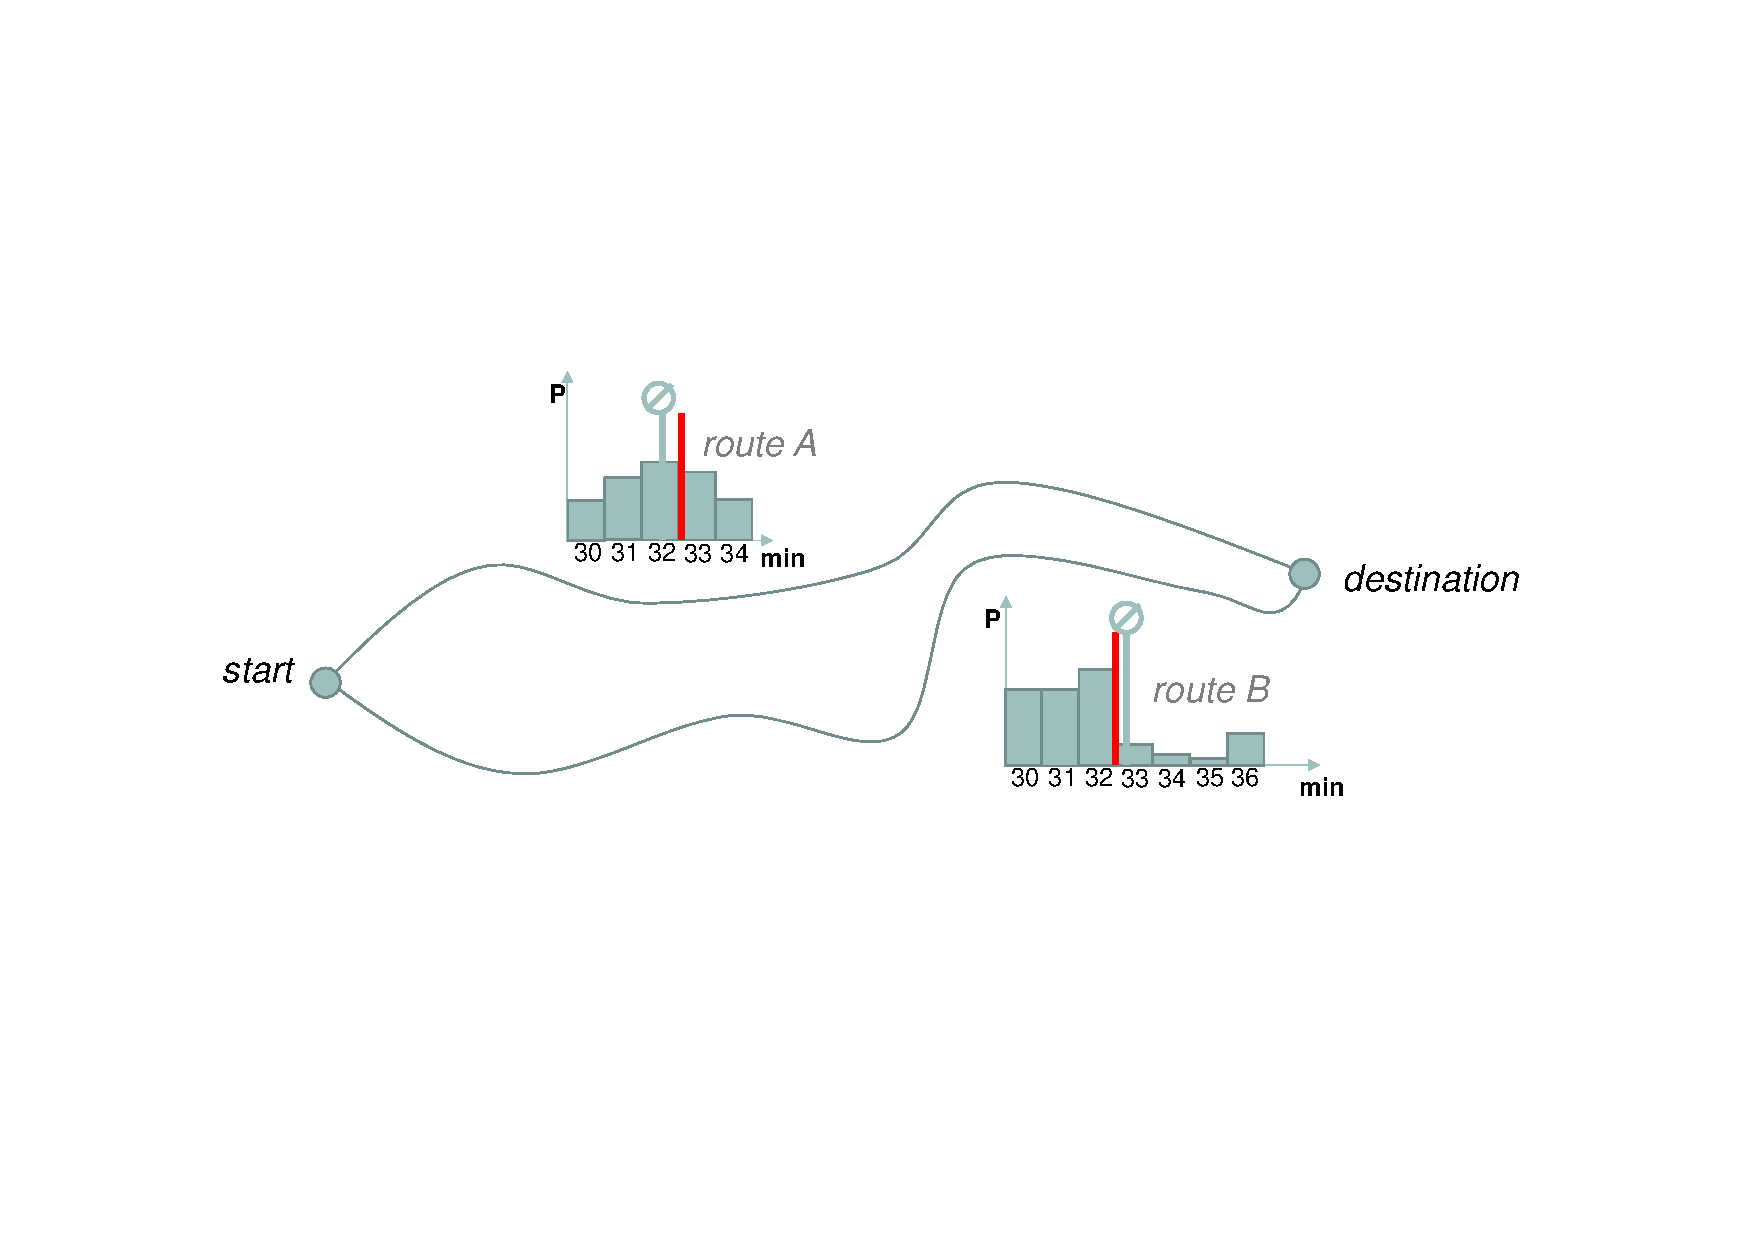
\includegraphics[width=0.90\columnwidth]{figures/motivation.pdf}
%     \caption{Probabilistic cost of two routes}
%     \label{fig:motivation}
% \end{figure}

\begin{figure}[t]
    \centering
    \subfigure[Deterministic result]{
        \label{fig:motivation1}
        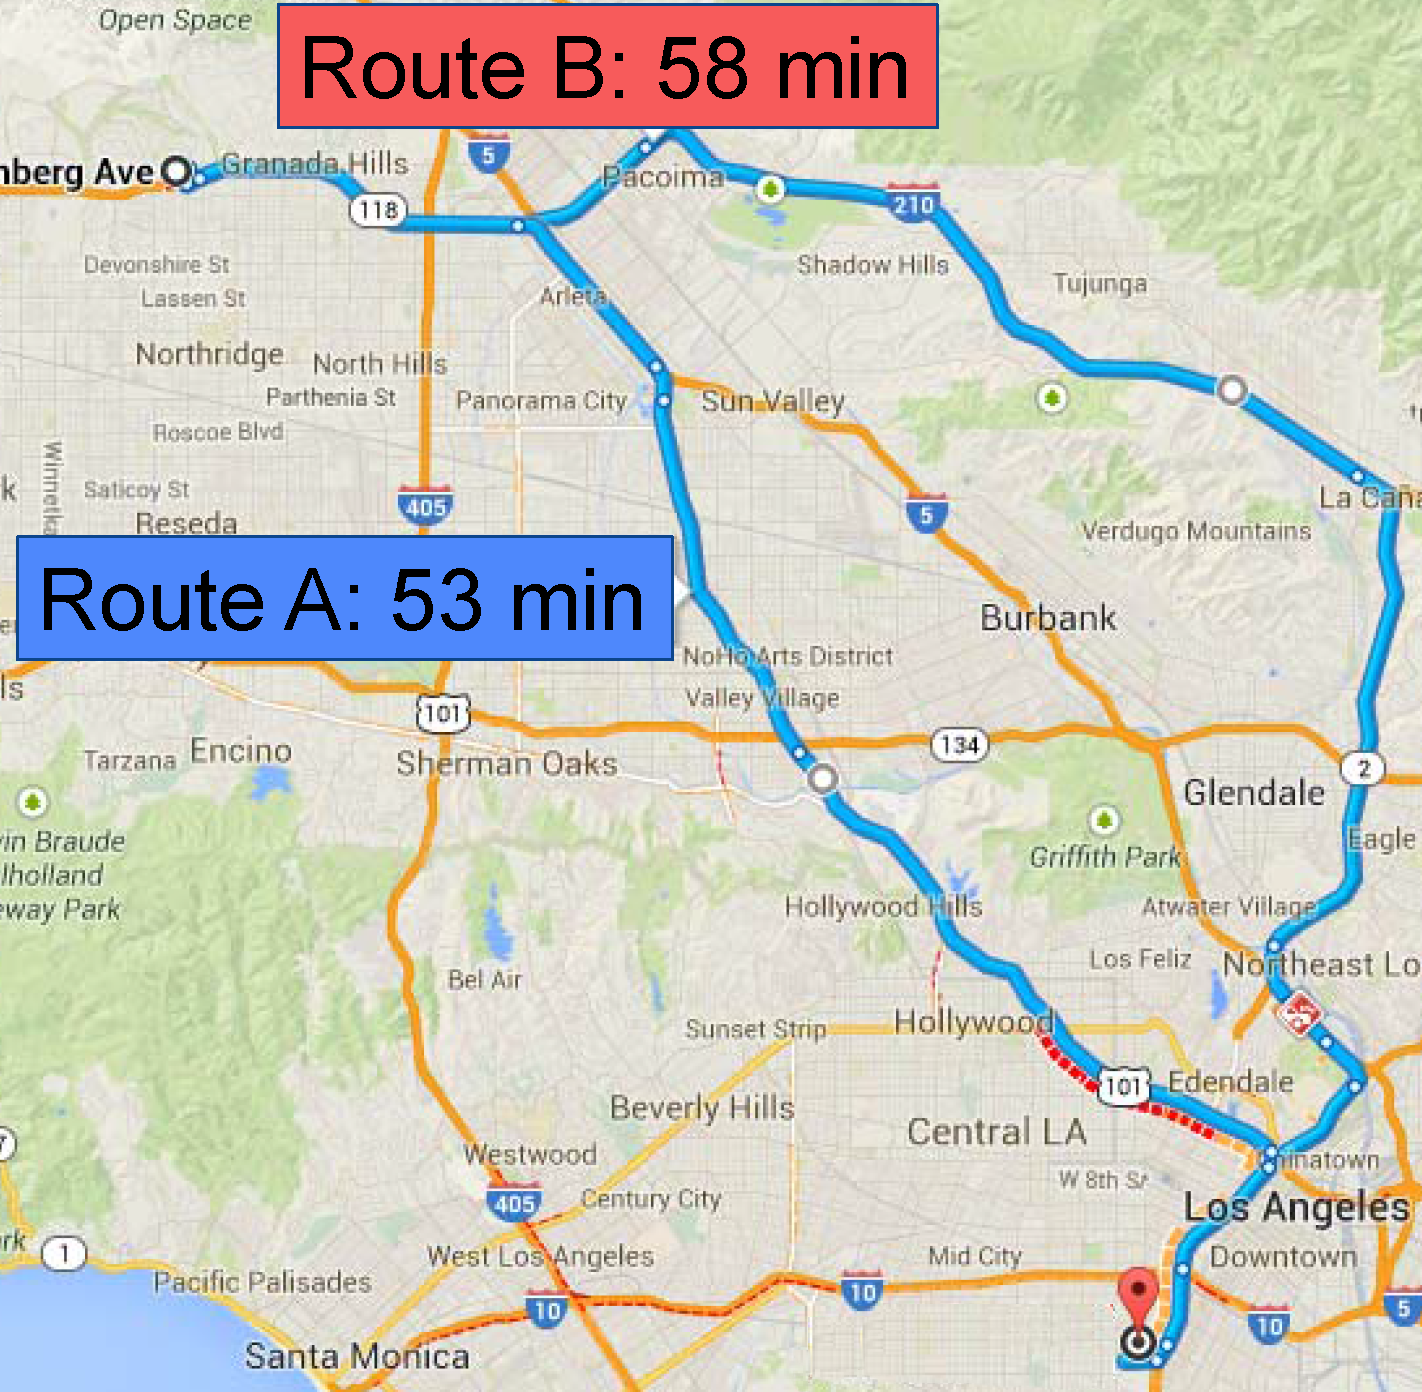
\includegraphics[width =
        0.38\columnwidth]{figures/motivation1_anonym.png} }
    \subfigure[Probabilistic result]{
        \label{fig:motivation2}
        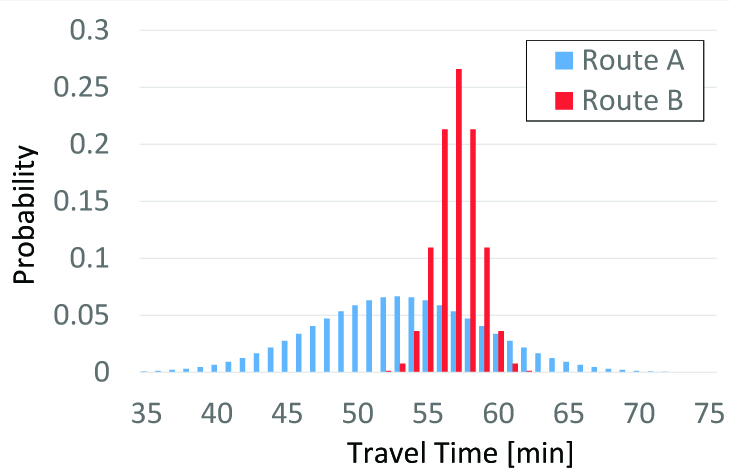
\includegraphics[width = 0.53\columnwidth]{figures/motivation2.jpg}
    }
    \vspace{-0.2cm}
    \caption{Estimated Travel Time of two paths}\label{fig:motivation}
    \vspace{-0.5cm}
\end{figure}

The above example shows that similar to other applications
\cite{Sarma08}, explicitly handling the uncertainty is better than ignoring it.
Correspondingly, we believe that taking the uncertainty of the travel time into account will
enable next-generation route planning applications by extending path queries to
probabilistic path queries, allowing for queries such as:  \textit{What are the
paths from my hotel to the airport whose travel time is at most 40 minutes with a probability of at least
95\%?}. 

% Recently, some studies have considered variations of the shortest-path
% problem under consideration of uncertainty (cf Section \ref{sec:related}) in
% the travel time. These studies reveal a plethora of useful scenarios and queries
% which can be enriched by confidence when taking this uncertainty into account.

With this goal in mind, in this work, we consider the problem of
computing the \textit{pdf} of the travel time for one given path. This
\textit{pdf} associates each possible travel time with the corresponding
probability that the vehicle will need this time for completing the route.
Specifically, we will make the following contributions:

\begin{enumerate}
  \item \label{item:1} It turns out that all existing approaches considering uncertainty in traffic
networks make the simplifying assumption that the probabilistic link travel
times (\textit{pltts}), i.e., the predicted time for each road segment, are
given. However, existing techniques on predicting link travel times provide a
single value estimation only or are not compatible with existing techniques for
computing the probabilistic link travel time of a path. Thus, there is a huge
lack in taking the uncertainty of predictions into account and estimating not
only accurate \textit{pltt} estimations but also possible correlations between them. We
will fill this gap by providing techniques that yield \textit{pltts} by taking historic
as well as real-time information into account.
  \item \label{item:2} Subsequently we focus on approaches for computing the
  probabilistic path travel times based on \textit{pltts}. After reviewing and categorizing the existing studies
 considering uncertainty in networks, we identify three basic characteristics
 (representation, time-dependency and correlation) and extract or adapt
 methods for all possible combinations of these characteristics for the ultimate
 goal of a fair and insightful comparison.
  \item The evaluation  of a probabilistic prediction is a daunting task.
  Neither expected distance measures nor goodness-of-fit methods nor primitive scoring
  functions are applicable. So far no evaluation of the accuracy for the
  methods in item \ref{item:2} has been performed. We propose adequate solutions to the evaluation problem and compare
  the accuracy of both the techniques in items \ref{item:1} and \ref{item:2} on
  a large real-world data set. Our results provide deep insights on the effect
  and functionality of all sub-modules.
\end{enumerate}

For the ultimate goal of providing this pipeline we avail ourselves of
techniques from database, transportation, weather prediction and statistics
research. One main question that this study will thus address is the
usefulness and validity of the consideration of uncertainty for route 
planning applications.
% 
% \begin{itemize}
%   \item We review and categorize existing work for shortest path algorithms on
%   uncertain traffic networks with a particular focus on the computation of the
%   uncertain travel time of one path.
%   \item We consider the problem of the parameter generation. This involves
%   estimating uncertain link travel times and correlations between these.
%   \item 
%   \item All experiments are carried out on a large scale real-world dataset
% \end{itemize}

% The remainder of this paper is structured as follows: In Section
% \ref{sec:problemdef} we formally define the problem setting and crucial notations. We review
% important related work in Section \ref{sec:related}. In Section
% \ref{sec:lttestimation} we propose methods for the probabilistic prediction of
% edge weights and correlations. How these predictions can be used in order to
% compute a prediction for a whole path is discussed in Section \ref{sec:methods}.
% We then discuss measurements for evaluating probabilistic predictions in Section
% \ref{sec:evaluate}. In a broad experimental setting we show both the validity of
% the proposed estimation methods for the link travel times and a comparison of
% the approaches in terms of efficiency and accuracy in Section
% \ref{sec:experiments}. Section \ref{sec:conclusion} concludes the paper.

% Figure \ref{fig:component} illustrates the components of this work.
% \begin{figure}[h]
%     \centering
%     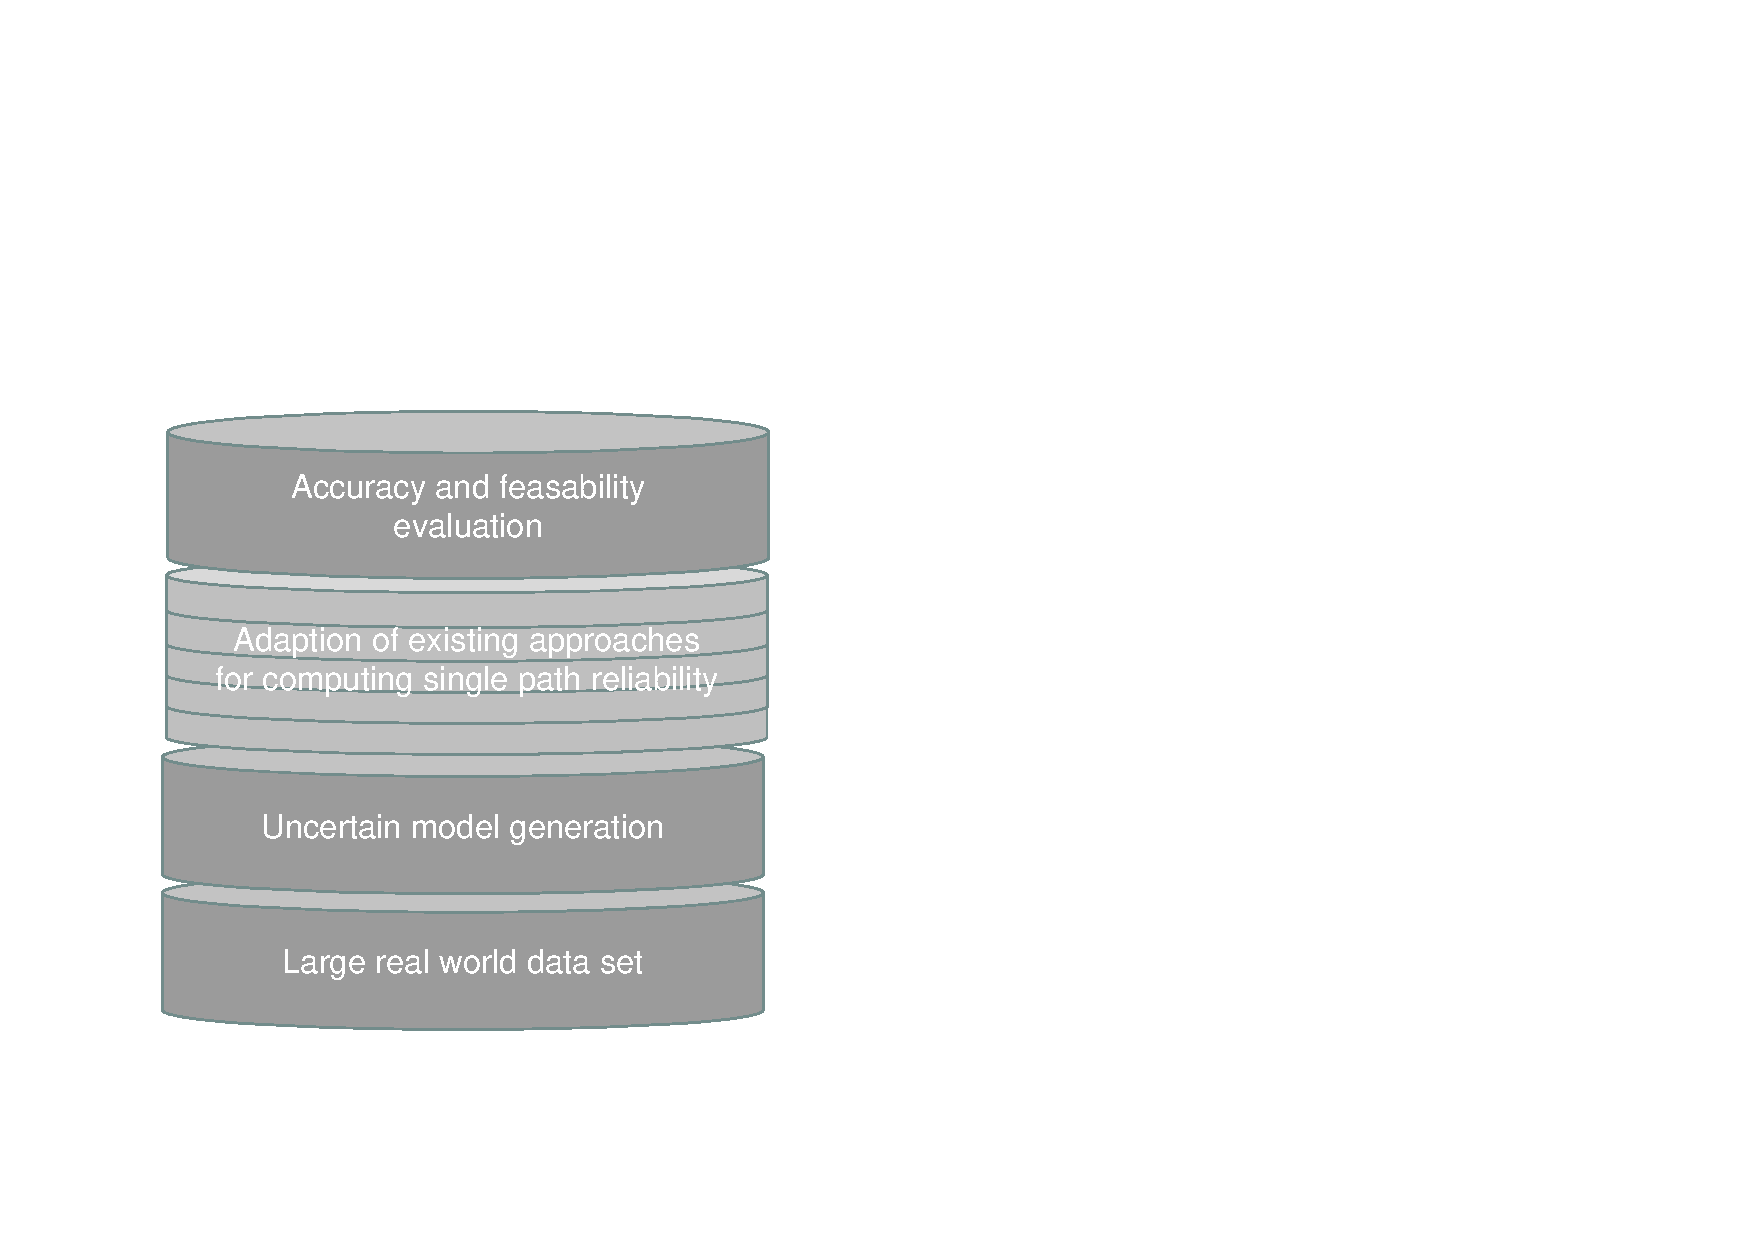
\includegraphics[width=0.50\columnwidth]{figures/contributions.pdf}
%     \caption{Components of this work}
%     \label{fig:component}
% \end{figure}


% ------Copy from \cite{NieWu09}-----------
% Another common definition of optimality in stochastic routing has to do with reliability, recognizing that a LET route (or
% policy) may be subject to high risks and therefore is not desirable to a
% risk averse
% traveler. For example, people tend to budget
% a large amount of time for travel when they plan for important events (e.g. job interviews). The key objective of routing in
% such a circumstance is to reduce the risk of arriving late rather than to minimize the expected travel time. In practice, how-
% ever, such risk averse behavior leads to excessively conservative time budgets. It is therefore necessary to both guarantee
% reliable on-time arrival and avoid unnecessary waiting. This paper precisely addresses the above problem.
% ------Copy end -----------
\section{Problem Definition}
\label{sec:problemdef}
In this section, we define the terminologies used in the paper and give a formal definition of the problem under consideration.

\begin{definition} [Probabilistic link travel times]
In a road network, for every link $(i, j)$ we define the probabilistic link travel time of link $()i,j$, $c_{ij}^t(x)$, as the probability of taking $x$ seconds for a vehicle to traverse link $(i,j)$ starting at time $t$.
\end{definition}

The link travel times are thus time dependent and differ depending on the arrival time of the vehicle at that starting point of the link. Additionally we consider $c_{ij}^t$ to be a random variable with $f_{ij}^t$ representing its \textit{pdf}.

\begin{definition} [Route pdf (\textbackslash pmf)]
Assuming $p_{sd}$ represents a path starting from point $s$ and ending in point $d$, we define $\pi_{sd}^t$ as the random variable representing the travel time on $p_{sd}$ when we start at time $t$. Accordingly, the route pdf, $J_{sd}^t(x)$, gives the probability of taking $x$ seconds for a vehicle to traverse $p_{sd}$ starting at time $t$.
\end{definition}

The problem considered in this paper is how to  accurately estimate $c_{ij}^t$.

%Consider a directed and connected transportation network $G(V, E, S)$ consisting of a set of nodes $V$, a set of links $E$ and a probability distribution $S$ describing the statistics of the link travel times. The link travel time $c_{ij}^t$ of an edge  $(i,j) ((i,j) \in E, i, j \in V)$ defines the time it takes for a vehicle to traverse the edge when starting at time $t$ at node $i$. The link travel times are thus time dependent and differ depending on the arrival time of the vehicle at that edge. Additionally we consider $c_{ij}^t$ to be a random variable with $f_{ij}^t$ representing its \textit{pdf}. The problem considered in this paper is how to obtain the \textit{pdf} for $c_{ij}^t$. Later on, such \textit{pdf} is used to build a \textit{pdf} for an entire route. If $p_{sd}$ represents a path from node $s$ to node $d$ we call $\pi_{sd}$ the random variable representing the travel time on $p_{sd}$. 

%Existing studies so far focused on different algorithms combining given \textit{pltts} and forming a \textit{pdf} for the entire route. However, to the best of our knowledge none of these studies have considered generating the \textit{pltts} themselves. Hence, none of these studies are able to examine the whole pipeline from the raw real-data to the probabilistic outcome and evaluate them properly - which poses several additional challenges. Towards this end, in addition to proposing techniques to generate \textit{pltts}, we also see this work as a study on how to evaluate probabilistic approaches on uncertain data in a real-wold setting in general. With this paper, we will focus on the following three specific problems:

%\textbf{(1) Probabilistic prediction of edge weights:} We develop techniques that compute probabilistic link travel times. Specifically, we aim at obtaining a \textit{pdf} (or \textit{pmf}) representing $c_{ij}^t$ based on the following data:

%\begin{itemize}
%\item The graph of the road network to consider $G(V,E)$.
%\item For each edge $(i,j) \in E$ historical data about the   link travel time $c_{ij}^t, t \in H = \{-L\phi, (L+1)\phi, \ldots, -\phi\}$, where $\phi$ is the smallest considered time unit and $L \in \NN$.
%\item For each edge $(i,j) \in E$ the current link travel time $c_{ij}^0$.
%\end{itemize}

%\textbf{(2) Technical analysis of existing work:} We classify existing approaches for computing the probabilistic path travel time $\pi^t_{sd}$ according to some of their basic characteristics. Then we apply the different \textit{pltt} generation techniques proposed on this paper to these approaches to evaluate the significance of using a good Vs. bad \textit{pltt} generation technique on the overall outcome.

%\textbf{(3) Evaluation of probabilistic predictions:} The evaluation and comparison of different approaches has to be carried out with a selected repertory from the statistical toolbox. The main challenge here is that the outcome of the methods for a specific starting time $t$ and a path  $p_{sd}$ is a \textit{pdf} over the estimated path travel time $\pi^t_{sd}$. Comparing the outcome with the true travel time over several trials has the challenge that $\pi^t_{sd}$ differs for different starting times. We thus propose a statistical test that enables us to evaluate these outcomes.

% \section{Categorization of Approaches} 
% The above problem statement however is very general and the existing works to
% solve this problem each use a specialized model for $S$. Generally they can be
% categorized by the following three attributes: model for the link travel times,
% consideration of time-dependency and modelling of correlations.
% 
% \subsection{Model for Link Travel Times}
% 
% 
% \subsection{Time Dependency}
% Especially in road-networks time-dependency is a crucial feature which allows
% for a much more precise estimation of the overall travel time. This is obvious
% since the conditions of a road network (including density of vehicles, traffic
% jams, construction sites, accidents) may change rapidly and effect the single
% link travel times drastically. Depending on time $t$ of the day the
% travel time $c_{ij}^t$ for a road segment may thus be represented by a
% different \textit{pdf} (e.g. travel time for the same road segment may be represented either by the \textit{pdf} shown in Figure
% \ref{fig:discrete} for Sundays or by the \textit{pdf} shown in Figure
% \ref{fig:traffic} during rush hours on weekdays).
% 
% \begin{figure}[h]
%     \centering
%     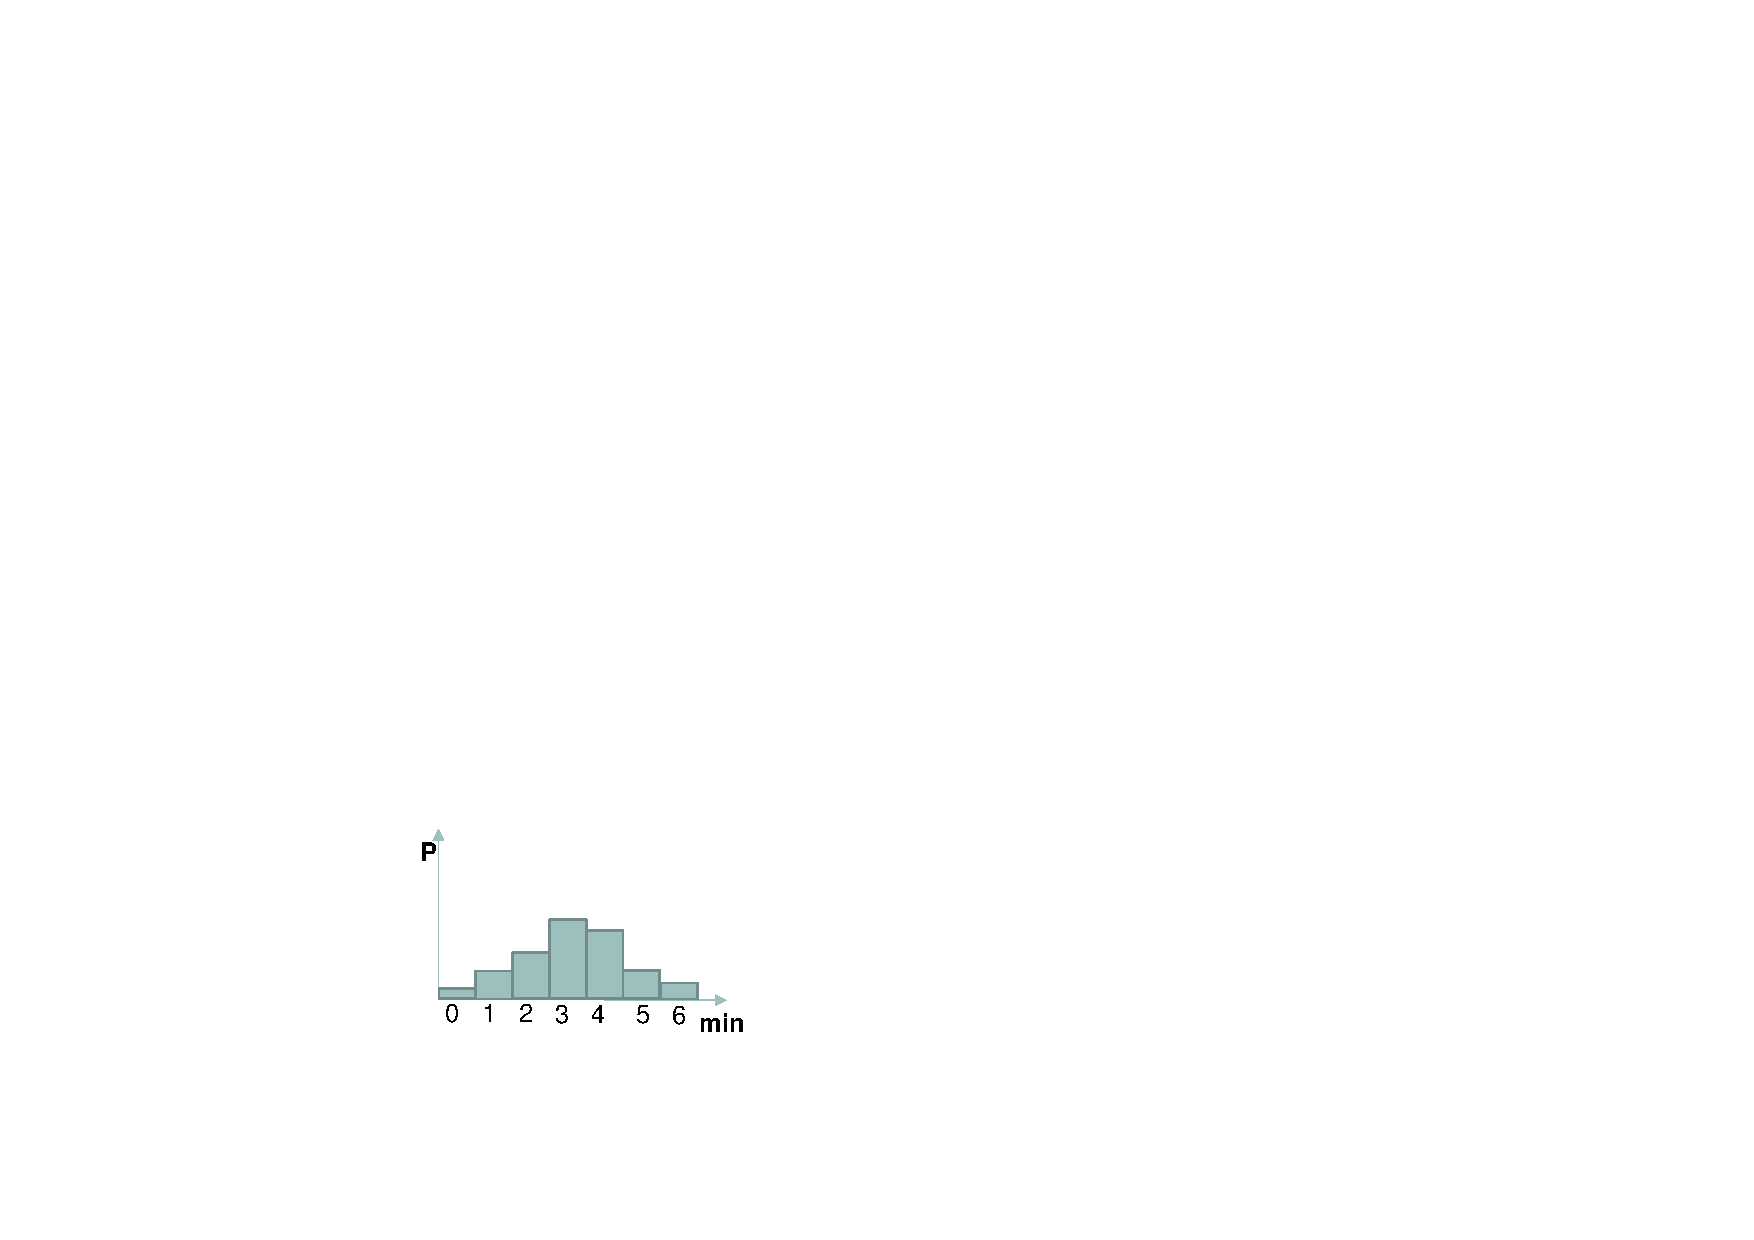
\includegraphics[width=0.5\columnwidth]{figures/pdf_traffic.pdf}
%     \caption{link travel time at rush hour}
%     \label{fig:traffic}
% \end{figure}
% 
% \subsection{Link Travel Time Correlations}
% The last characteristic is the modelling of correlations between link travel
% times. It is possible to treat the link travel times of different road segments
% (edges) as independent random variables. However on a real-world traffic
% network, it might be more realistic to assume correlated link travel times. For
% example if there is a traffic jam on on road segment yielding high travel times
% then it is likely that the subsequent road segment is also jammed and the travel
% time is also high. To model the correlation between random variables, there
% exist several approaches which will be reviewed in the following section.



\section{Probabilistic Link Travel Times}
\label{sec:lttestimation} 
The prediction of an event is usually tainted with uncertainty. Therefore, when predicting link travel times it is not possible to produce an accurate prediction, since there are too many influencing factors like road conditions, accidents, weather, time of the day, day of the week or season. The methods we propose, produce a probabilistic prediction which includes all the effects that have been observed before (historic data) and are influencing the traffic flow right now (current data). For example if a street segment has often been the place of an accident (e.g., every other day between 9.00am and 10.00am) then the historical data will capture this effect and assign a high probability (e.g., 50\%) to the prediction that the travel time on that segment will be higher than usual. In this section we will develop three approaches to estimate probabilistic link travel times and correlations between them.

Before we continue, we need to introduce and explain a few concepts that will be used throughout this section. \textit{Start time} $(t_s)$, is the time for which we want to predict the travel time. For example, if we want to know how long it will take to travel from point $A$ to point $B$ if we leave at 8:00am, then the \textit{start time} will be 8:00am. \textit{Query time} $(t_q)$, is the time at which we are making the prediction. For example, if the current time is 7:00am and we want to know how long it will take to travel from point $A$ to point $B$ if we leave at 8:00am, then the \textit{query time} will be 7:00am. As it was seen in this example, \textit{start time} and \textit{query time} necessarily are not the same. We call the difference between the two the \textit{prediction time} $(t_p)$.

\textbf{Probabilistic Link Travel Times: } The probabilistic link travel time of a link $(i,j)$ at time $t$, $c_{ij}^t$, can be represented with two models; discrete or continuous.

To represent the link travel time $c_{ij}^t$ with a continuous \textit{pdf}, an appropriate function is needed. Recent studies suggest that in road networks, the link travel times are normally (e.g. \cite{Seshadri10}) or gamma (e.g. \cite{Zockaei13}) distributed. \cite{Moschopoulos85} shows how to compute the sum of several gamma distributed random variables. The methods in \cite{Moschopoulos85} can be combined with the same approaches discussed here to compute route pdfs for routes consisting of links with gamma distributed travel times. In this study we only focus on link travel times that are normally distributed. In the case of a normal distribution, the random variable $c_{ij}^t$ is characterized by a mean $\mu_{ij}^t$ and a standard deviation $\sigma_{ij}^t$.

In the discrete case, the link travel time is represented by a discrete probability mass function. Therefore, the time domain has to be discretized. The simplest discretization scheme, known as b-discrete, divides the time domain $T = \{t | t = n\cdot \phi \wedge n \in \NN \}$ evenly into intervals of length $\phi$. The corresponding probability mass function $F_{ij}$ of link travel time $c_{ij}$ reads:

\begin{equation}
	F_{ij}(b) = \begin{cases}\int_b^{b+\phi}f_{ij}(w)dw \qquad b =
	0,\phi,\ldots, (L-1)\phi\\
	\int_b^{\infty}f_{ij}(w)dw \qquad b =
	L \phi\\
	0 \qquad otherwise
	\end{cases} 
\end{equation}
where $L \phi$ is the maximal considered time horizon in the future.

\begin{figure*}
    \centering
    \subfigure[9:00am]{
        \label{fig:900}
        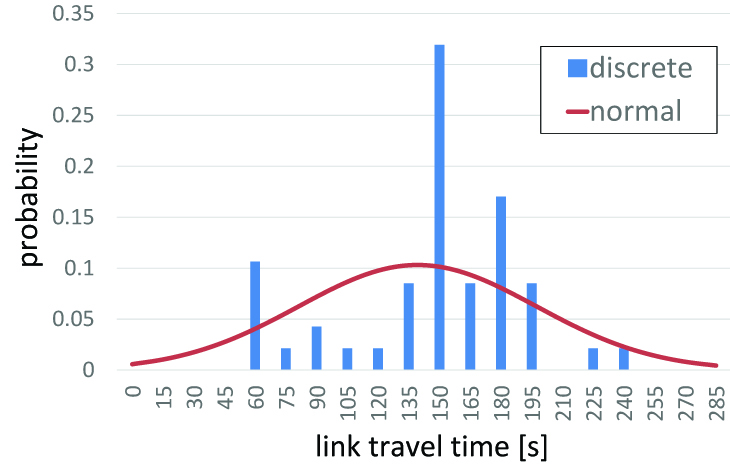
\includegraphics[width = 0.6\columnwidth]{figures/ltt_0900.jpg}
    }
    \subfigure[12:00pm]{
        \label{fig:1200}
        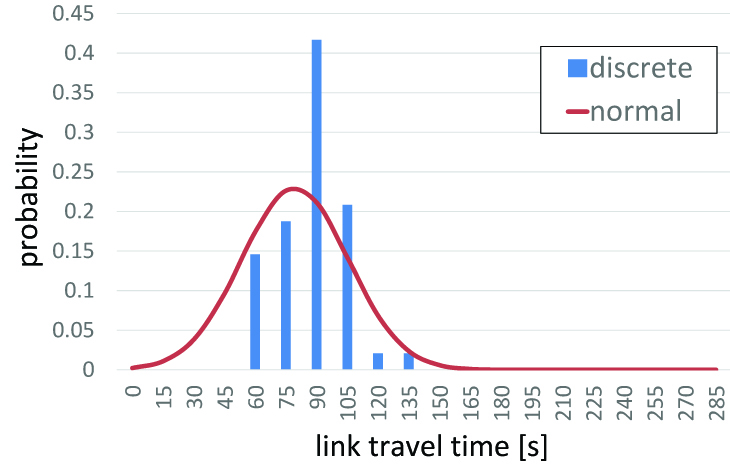
\includegraphics[width = 0.6\columnwidth]{figures/ltt_1200.jpg}
    }
    \subfigure[6:00pm]{
        \label{fig:1800}
        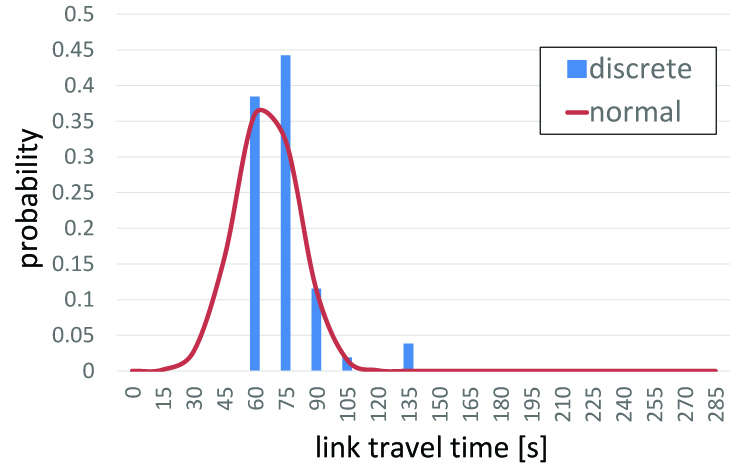
\includegraphics[width = 0.6\columnwidth]{figures/ltt_1800.jpg}
    }
    \caption{Historical model for a street segment for different times of a
    Monday}\label{fig:ltt}
\end{figure*}

In the remainder of this section, we will discuss our techniques to generate probabilistic link travel-times.

\subsection{Prediction through Historical Data}
\label{subsec:historical}
To obtain a \textit{pdf} representing $c_{ij}^{t_s}$ for a start time $(t_s \geq t_q)$ a simple approach is to use the available historical data. We define the set of historical data as $H = \{h | h < t_q\}$. Let us note that the link travel time $c_{ij}^h$ where $ h < t_q$ is not a random variable but a certain value which is known. In order to predict the travel time for time $t_s \geq t_q$ more accurately, we only consider a subset of historical data, $H^{t_s} \subset H$, with similar characteristics to time $t_s$. For example, if we want to predict the behaviour of edge $(i,j)$ at 9:00am for the next Tuesday, an adequate set $H^{t_s}$ might consist of data points $h$, where $h$ is 9:00am on a Tuesday in the last year. The travel time $c_{i,j}^h$ corresponding to last Friday 10:00pm might on the other hand, not be valuable in the prediction.

How to choose a set $H^{t_s}$ highly depends on the characteristics of the underlying traffic network. We use the results in \cite{Pan12} for choosing the appropriate $H^{t_s}$ for each start time. For a specific \textit{time of day} during a weekday, $H^{t_s}$ consists of data points corresponding to the same \textit{time of day} during \textbf{\textit{any}} weekday. For example, if the start time is 9:00am on this Tuesday, $H^{t_s}$ will consist of data points at 9:00am during Mondays, Tuesdays, Wednesdays, Thursdays and Fridays. The assumption is that traffic patters during weekdays are similar. More details can be found in \cite{Pan12}.

For continuous representation of the link travel time, we assume normal distribution with the following parameters
\begin{gather}
	\mu_{ij}^{t_s} = \frac{1}{|H^{t_s}|}\sum_{h\in H^{t_s}} c_{i,j}^h\\ 
	(\sigma_{ij}^{t_s})^2 = \frac{1}{|H^{t_s}|}\sum_{h\in H^{t_s}} (c_{ij}^h-\mu_{ij}^{t_s})^2\\
	\rho_{ij-kl} = \frac{\sum_{h\in H^{t_s}} (c_{ij}^h - \mu_{ij}) (c_{kl}^h -
	\mu_{kl})}{(|H^{t_s}-1| \sigma_{ij} \sigma_{kl})}
\end{gather}

where $\rho$ is the Pearson correlation coefficient \cite{Soper17}

For the case of discrete representation through a \textit{pmf} we set

\begin{gather}
  F_{ij}^{t_s}(b) = \frac{1}{|H^{t_s}|}\sum_{h\in H^{t_s}} I(\lceil c_{ij}^h \rceil^\phi= b)
\end{gather}

where $\lceil x \rceil^\phi$ rounds $x$ up to the next multiple of $\phi$ and $I(c_{ij}^h = b)$ is an indicator variable which is 1 if $c_{ij}^h = b$ and 0 otherwise. The \textit{pmf} of each edge is thus given by a histogram assigning for each possible travel time of the edge a probability corresponding to its proportional occurrence in the historical data. 

\cref{fig:ltt} shows the discrete and continuous models of a typical inbound street segment of the network with a length of 1 mile for different times of the day. Based on the observation of historic patterns, in the morning a lot of traffic passes through this link. More traffic, intuitively, implies a higher probability of accidents which explains the rather large variation in the link travel time. At noon the traffic is reduced and in the evening the link travel time has the least amount of traffic, yielding the fastest travel time and in this case also the smallest variance. The figure also shows that the use of a normal distribution might not always adequately represent the link travel time.

We end this subsection with a note on \textit{query time} and \textit{prediction time}. When only historic data is used for prediction, the concept of prediction time becomes irrelevant. This means that if we are predicting for start time set to 9:00am today and we only use historic data, whether the query time is 7:00am or 8:00am does not make any difference since we only use $H^{t_s}$ corresponding to the start time to build the model. Prediction time and query time become important once we take the \textit{current situation} into account when building the prediction model which we will discuss in the following. 

\subsection{Historical Data and Current Situation}
The technique discussed in \cref{subsec:historical} provides link travel time distributions only based on historical data. These estimations may be a good choice if the start time $t_s$, for which the link travel time has to be predicted, is reasonably far (e.g., more than several hours) in the future. However, it may not be sufficient to capture current (and near future) traffic conditions with high confidence. For example, if we want to predict the travel time for 5 minutes later, the current situation of the road network might be more relevant than the historic data. Therefore, we present two parameter estimation methods, incorporating both, the historical as well as the current link travel times of edges.

\subsubsection{Prediction through Linear Interpolation}
\label{subsec:LI}
The intuition of this approach is that 
\begin{itemize}
  \item for a start time $t_s$ which is far in the future, the historical prediction (cf \cref{subsec:historical}) is expected to yield a good prediction performance and
\item for the start time $t_s = t_q$, the current situation yields the best "prediction".
\end{itemize}

Thus, for a start time $t_s$ which is in the relatively near future, we argue that both, the historical as well as the current situation should influence the prediction. The closer the time $t_s$ is to $t_q$ (smaller prediction time) the more weight the current situation should have and vice versa. As the prediction time increases, we eventually get to a point where the current situation should loose it's influence. Towards this end we define a threshold parameter $\tau$, which defines the time-horizon in which the current situation has an influence on the prediction. Using a small time horizon $\tau$ is basically valuing the historic data, whereas setting $\tau$ to a larger value puts more weight on the current situation. We also define $\theta \in [0,1]$ as the relative importance of the current situation in the estimation. $\theta$ depends on the prediction time and is computed as:
\begin{equation}
\theta = min \{\frac{t_s-t_q}{\tau}, 1 \}
\end{equation}
where, as explained earlier, $t_s-t_q$ is the prediction time.

For continuous representation of link travel times, we estimate the parameters of the normal distribution as:

\begin{gather}
	\mu_{ij}^{t_s} = \left(\theta\cdot\frac{1}{|H^{t_s}|}\sum_{h\in H^{t_s}} c_{i,j}^h \right)
	+ \left(1-\theta\right)\cdot c_{i,j}^{t_q}\\
	(\sigma_{ij}^{t_s})^2 = \theta^2 \cdot \frac{1}{|H^{t_s}|}\sum_{h\in H^{t_s}}
	(c_{ij}^h-\mu_{ij}^{t_s})^2
\end{gather}

In particular, we perform a linear interpolation between the current link travel time, and the summarized historical link travel time in order to find the link travel time to be estimated. \cref{fig:interpolation} illustrates this concept, where  $\theta = 0.5$ and thus the expected value of the prediction is the average of the current situation and the predicted value by the historical approach. Accordingly, the standard deviation of the historical prediction is cut by half.

\begin{figure}[h]
    \centering
    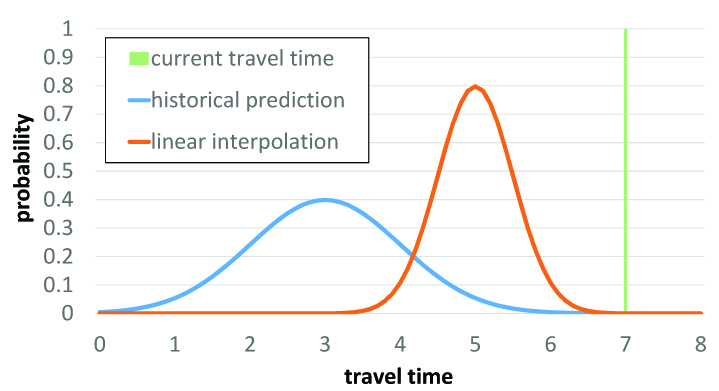
\includegraphics[width=0.80\columnwidth]{figures/tt_interpolation.jpg}
    \caption{Linear interpolation of ltt}
    \label{fig:interpolation}
\end{figure}

In the case of discrete link travel times, we adapt the same concept and obtain the following parameters.

\begin{gather}
F_{ij}^{t_s}(b) = \frac{1}{|H^{t_s}|}\sum_{h\in H^{t_s}} I(\lceil\theta \cdot 
c_{ij}^h + (1-\theta)\cdot c_{i,j}^{t_q}\rceil^\phi = b)
\end{gather}

where $\lceil x \rceil^\phi$ rounds $x$ up to the next multiple of $\phi$ and $I()$ is the indicator function.

\subsubsection{Prediction through Similar Historical Data}
\label{subsec:SH}
The third and final approach we propose is based on the idea that the current situation is a crucial indicator of how the travel time of a link will develop in the future. In this approach we use the current situation to further restricts the set $H^t_s$. Specifically we only include times $h \in H^t_s$, for which link $(i, j)$ had a travel time similar to the current situation at time $h-(t_p)$. In this context, we define similarity by a percentage threshold $\lambda$, which represents the deviation from the current travel time. To illustrate this idea, we provide an example. Assume we are predicting the travel time for link $l$ where the $t_q=$ 7:00am and $t_s=$ 8:00am. We only consider the data points at 8:00am from days where the traffic at 7:00am was similar to today. For example, if the current travel time over link $l$, is 5 minutes and $\lambda = 0.2$, we only consider days where the travel time over link $l$ is somewhere between 4 minutes and 6 minutes.

We can formally define the further restricted set $H_{i,j}^{t_s}$ as:

\begin{equation}
H_{i,j}^{t_s} = \{h|h \in H^{t_s} \wedge \left| \frac{c_{i,j}^{t_q} - c_{i,j}^{h-t_p}}{c_{i,j}^{t_q}} \right| \leq \lambda \}  
\end{equation}

The value of $\lambda$ affects the prediction result. Setting $\lambda$ too small might result in not enough sample points. This can cause problems like over fitting the model. On the other hand setting $\lambda$ too large yields the historical prediction approach. In \cref{sec:experiments} we test with different values of $\lambda$ to find the optimal value for this parameter. 



\section{Route Reliability Computation}
\label{sec:methods}
In this section we present a classification of existing approaches for computing route pdfs. Towards this end, we identified three basic characteristics of these algorithms which become the basis of our classification; link representation, time dependency and link correlation. Different algorithms model link travel times as either discrete or continuous distributions, they can consider the network time dependent or static and finally they would either consider correlation between the travel time of different links or look at them independently. \cref{tab:methods} summarizes the existing work on route pdfs (\textbackslash pmfs) based on the three attributes we presented here. A brief description of each work is presented in \cref{sec:related}.

\begin{table}
\centering
\begin{tabular}{| l || l | c | c | c | c|}
\hline
Ref. & Method & Link model & Time-dep. & Correl. \\
\hline    \hline
\cite{Frank69} & ConStaInd & continuous  & no & no\\ \hline
               & DisStaInd & discrete & no & no\\ \hline
               & ConTimInd & continuous & yes & no\\ \hline
\cite{Miller-Hooks98,Miller-Hooks00, Nie09b} & DisTimInd & discrete & yes & no\\ \hline
\cite{Seshadri10, Zockaei13,Bi-Yu13} & ConStaCor & continuous & no & yes\\ \hline
\cite{Nie06,Hua10,Fan05} & DisStaCor & discrete & no & yes\\ \hline
\cite{Dong12} & ConTimCor & normal & yes & yes\\ \hline
\cite{Nie09a} & DisTimCor & discrete & yes & yes\\ \hline
\end{tabular}
\caption{Models considered in this work}
\label{tab:methods}
\end{table}

To fully evaluate the techniques in \cref{sec:lttestimation} for computing \textit{pltts}, we need to apply each technique to existing algorithms and check the accuracy of the resulting route pdf (\textbackslash pmf). Also, since there has not been any study to compute \textit{pltts}, it has not been possible to compare the performance of these algorithms based on real world datasets. Following, we briefly explain a few classes of the algorithms presented in \cref{tab:methods} which we later use in our experiments. The selection of the classes is such that give us the ability to compare the effectiveness of the attributes used to classify these algorithms. For example by comparing the results of \textbf{ConStaInd} (\textbf{Con}tinuous, \textbf{Sta}tic, \textbf{Ind}ependent) with the results of \textbf{ConStaCor} we can find out whether considering link correlations increases the accuracy of the final pmf or not.

\textbf{ConStaInd: }Assuming link travel times are normally distributed and independent, the path travel time is also a random variable which is normally distributed with a mean and a variance, given by

\begin{gather}
\label{eq:normal}
	\mu_{p} = \sum_{(i,j)\in p} \mu_{ij} \text{ and } \sigma_{p}^2 =
	\sum_{(i,j)\in p} \sigma_{ij}^2 
\end{gather}

where $(i,j)$ represent links on path $p$.

\textbf{DisStaInd: } Given the \textit{pmf} $F_{ij}$ of the link travel time for the link $(i,j)$ we can compute the \textit{pmf} $J_{sj}$ of the path travel time of path $p_{si}$ extended by the link $(i,j)$ by using the poisson-multinomial recurrence.

\begin{equation}
\label{eq:pmr}
	J_{sj}(b) = \sum_{h=0}^b J_{si}(b-h) F_{ij}(h)  , \forall b = 0, \phi,\ldots, L
	\phi
\end{equation}

This equation can be computed efficiently by starting with the first link $(s,i)$ of the path $p_{sd}$ and its corresponding \textit{pmf} $F_{si}$. The adjacent link $(i,j)$ is considered next. The \textit{pmf} $J_{sj}$ is computed according to Equation \ref{eq:pmr} and the process repeats with the next adjacent link until node $d$ is reached. 

\textbf{DisTimInd: } Let $F_{ij}^t$ be the \textit{pmf} describing the link travel time of the link $(i,j)$ at time $t$ and $J_{si}$ be the path travel time for a path $p^{si}$. We assume that the route starts at $s$ at $t = t_c = 0$ then:

\begin{equation}
\label{eq:pmr2}
	J_{sj}(b) = \sum_{h=0}^b J_{si}(b-h) F_{ij}^{b-h}(h)  , \forall b = 0,
	\phi,\ldots, L
	\phi
\end{equation}

Similar to Equation \ref{eq:pmr} we can build an incremental algorithm upon this equation until node $d$ is reached.

\textbf{ConStaCor: } We manage to capture link correlations for the continuous representation by extending Eq. \ref{eq:normal} as follows:

\begin{gather}
\label{eq:normal2}
	\mu_{p} = \sum_{(i,j)\in p} \mu_{ij}, \\
	\sigma_{p}^2 = \sum_{(i,j)\in p} \sigma_{ij}^2 +\sum_{(i,j)\neq(k,l)\in p}
	\rho_{ij-kl}
	\sigma_{ij} \sigma_{kl}
\end{gather}

This compact representation of the correlation of link travel times is only possible due to the assumption of normally distributed link travel times. 
\section{Evaluating Probabilistic Predictions}
\vspace{0.2cm}
\label{sec:evaluate}
Evaluating the accuracy of probabilistic results is a task that has been either
over simplified or brushed under the carpet by many studies, focusing on the
technical aspects of managing uncertain data. However, we argue that this part
is crucial in order to justify the use of the uncertain aspects in the data,
rather than performing the traditional approaches for data cleaning (e.g., using the expected prediction
time). The evaluation of probabilistic prediction models for nominal values
(e.g., travel time) is a non-trivial problem that will be reviewed in this
section.

The problem statement is as follows: Let A be a prediction model that is able
to provide a probabilistic prediction $f_A^t$ of a value $v^t$ for a
time $t$ in the future and $f_A^t$ be a \textit{pdf} assigning a probability to
each possible value of $v^t$. Furthermore, let B be a prediction model which predicts
$f_B^t$ for the same value $v^t$. Our goal is to determine which of the two
models yields a better probabilistic prediction.

Two statistical methods are considered to be relevant to this problem:
goodness-of-fit tests \cite{Taylor97} and scoring rules \cite{Bickel07}. The
goodness-of-fit test describes how well a statistical model fits a set of
observations.
Measurements of goodness-of-fit typically summarizes the discrepancy between
observed values and the values expected under the model in question. An example is the
Pearson's Chi-Square test \cite{Pearson00}, which can be used as a goodness-of-fit
test for a given \textit{pdf} $f$, which represents the theoretical behavior of
a random variable $v$, and an observed frequency distribution (sampled values)
from that variable. The test returns the probability of observing this frequency
distribution (or a frequency distribution with a higher difference) under the
assumption that the true distribution of $v$ follows $f$. Obviously this measure
might be used in order to compare two models $f_A$ and $f_B$. The main
difference of this setting is that the prediction is in our case time-dependent
and changes additionally depending on the current situation of the traffic on
an edge. Thus we are not able to draw a sufficiently large number of samples
that may validate either one or the other model.
Scoring models on the other hand are designed to evaluate probabilistic
prediction models that are time dependent. Fields of application are weather
forecasting or betting games. The most prominent representative is known as the
Brier scoring rule \cite{Brier50}, which is described as follows. Let $f^t$ be a
probabilistic prediction model (e.g., a probability mass function) for a
variable, whose true value $v^t$ is one of several classes $C$ (e.g., ``tomorrow
is sunny (75\%) or rainy (25\%)), then for one specific $t$ the Brier scoring
rule returns:

$$
	S^{Brier}(f^t, v^t) = -\sum_{c \in C} (f^t(c) - I(v^t = c))^2
$$
where $f^t(c)$ represents the probability that is assigned to class $c$ and
$I(v^t = c)$ returns 1 if the true value of $v^t$ is equals $c$.
Intuitively, this scoring function gives a reward dependent on the
probability that the probabilistic prediction model assigns to the true value.
Summing up these rewards over several times $t \in T$ yields a score that is
higher the better the prediction model $f^t$ predicts the true probability
distribution of $v^t$ at each value of $t$:

\vspace{0.1cm}

$$
	S^\Sigma (f, v) = \sum_{t \in T} S^*(f^t, v^t)
$$

\vspace{0.1cm}

With this mechanism, it is possible to evaluate two probabilistic prediction
models $f_A$ and $f_B$ by comparing their corresponding rewards.
Scoring rules can also be used in our scenario, however they are originally
designed for categorical values (e.g., sunny, cloudy, rainy) rather than ordinal
values (e.g. travel time). Thus these scores are not sensitive to distance,
meaning that no credit is given for assigning high probabilities to values near
but not identical to the one materializing (e.g., the true outcome). For example
a probabilistic prediction model A, that predicts 5 minutes (90\%) or 6
minutes (10\%) and a model B that predicts 6 minutes (10\%) or 10 minutes
(90\%), both obtain the same score when the true travel time is 6 minutes. However, we argue that this approach
does not account for the ordinal nature of travel times since a true travel time
of 6 minutes is rather close to the highly probable 5 minutes of model A and a
good scoring rules should thus favor model A over B. For this reason we propose
to use the continuous ranked probability score (CRPS) which is defined as
follows \cite{Hersbach00}:

\vspace{0.1cm}

\begin{equation}
CRPS(f^t, v^t) = \int_{-\infty}^{+\infty} \int_{-\infty}^{x} f^t(y) dy - I(x
\geq v^t) dx
\end{equation}

\vspace{0.1cm}

CRPS thus expresses some kind of distance between the probabilistic forecast
$f^t$ and truth $v^t$. Another very useful property of CRPS is that it can be computed in
linear time (in the number of possible outcomes) in the case when $f^t$ is given
by a \textit{pmf} and has a closed form for the case where $f^t$ is given by a
normal distribution $\mathcal{N}$ with parameters $\mu$ and $\sigma$ \cite{Gneiting04}:

\vspace{0.1cm}

\begin{multline}
CRPS(\mathcal{N}(\mu,\sigma), v^t) = \sigma \left[ 2\varphi\left(\frac{x -
\mu}{\sigma}\right) - \frac{1}{\sqrt{\pi}} + \right. \\ \left.\frac{x -
\mu}{\sigma}\left(2 \Phi\left(\frac{x - \mu}{\sigma}\right) - 1 \right) \right]
\end{multline}

\vspace{0.2cm}

where $\varphi$ and $\Phi$ denote the probability density function and the
cumulative distribution function of a standard Gaussian variable. One advantage
of the CRPS is that it reduces to the mean absolute error (MAE) if the forecast
is deterministic. In practice, this makes it possible to compare an
ensemble forecast with a deterministic forecast of the same variable in a
consistent fashion. Since for the experimental evaluation we discretize the time
to 1 second (i.e., $\phi$ = 1 sec) this means that the CRPS score can be
interpreted as the mean absolute error of the predicted travel time in seconds.


%\newpage
\section{Experiments}
\label{sec:experiments}
\subsection{Dataset and Experimental Setting}
\subsubsection{Dataset}
\label{subsec:Dataset}
In our research center, at USC's IMSC, with our partnership with Los Angeles Metropolitan Transportation Authority (LA Metro), we maintain a big transportation data warehouse that fuses and analyzes a very large-scale and high-resolution (both spatial and temporal) traffic sensor data from different transportation authorities in Southern California, including California Department of Transportation (Caltrans), Los Angeles Department of Transportation (LADOT), California Highway Patrol (CHP), Long Beach Transit (LBT).  This data set includes both inventory and real-time data with update rate as high as every 30 seconds for freeway and arterial traffic sensors (9300 loop-detectors) covering more than 3500 miles, incidents  such as accidents, traffic hazards and road closures reported (approximately 400 per day) by LAPD and CHP, and ramp meters. We have been continuously collecting and archiving aforementioned datasets for the past three years. We use this real-world dataset to model and evaluate our techniques. To generate time dependent  travel times we spatially and temporally aggregate traffic sensor data by assigning interpolation points for each 5 minutes during a year that depict the travel-times on the segments of Los Angeles road network with 304,162 edges. Based on our observation, all roads are fairly un-congested between 9:00pm and 6:00am, and hence we assume static edge weights between those times. More detailed information regarding the dataset can be found in \cite{Jagadish14}.

\subsubsection{Experimental Setting}
All experiments were conducted on an Intel(R) Core(TM)2 Duo 3.16GHz PC running on Microsoft Windows 7. Methods were implemented in Java.

Predicting travel times in a rather static road network (with only marginal changes in the link travel times) is not very challenging and usually does not require a probabilistic prediction. For this reason we focused on rush hour times which imply more uncertainty and thus a much harder scenario for prediction. If not mentioned otherwise we used 8:00am, 9:00am, 4:00pm, 5:00pm and 6:00pm during the weekdays. These times were considered as the \textit{start time}, i.e. the time at which the user starts his route. According to the results from \cite{Pan12} and our own observations, traffic patterns are quite equivalent across weekdays. Consequently, we did not differentiate between predictions for different weekdays. This means for each start time, we consider data of 260 days (5 days per week, 52 week per year). \\
In our evaluation process, we used the k-fold cross validation (k=5) method to divide our data into test (test days) and training (training days) sets. In each fold, for each start time and each test day we investigated the following:
\begin{itemize}
  \item We used the data of the training days with one of our techniques to build a model for predicting the travel time of a link (\textbackslash route) at a specific start time. In case the \textit{current situation} is required for building the model, we can fetch it from the dataset.
  \item For the specific test day and start time, we find the \textit{actual} travel time over the link (\textbackslash route) from the dataset.
\end{itemize}
Both of these outcomes are then used to compute a CRPS score as defined in Section \ref{sec:evaluate}, which is then averaged over all folds and trials. For all discrete models we discretize the time into 1 second intervals.

\subsection{Probabilistic Link Travel Time Prediction}
\label{subsec:pltt_prediction}
In our first set of experiments we evaluate the prediction quality of the following three proposed approaches:
\begin{itemize}
  \item HP: Prediction purely based on historical data as described in \cref{subsec:historical}.
  \item LI: Prediction based on linear interpolation between the current situation and the prediction based on historical data as discussed in \cref{subsec:LI}.
  \item SH: Prediction based on historical data with behavior similar to the current situation as proposed in \cref{subsec:SH}.
\end{itemize}

We tested all techniques over 50 links which are chosen randomly from all around the road network explained in \cref{subsec:Dataset}. The links we chose for these experiments are ~1 mile long and all are on highways. The link selection process was such that we had 6-8 links from each major highway in the L.A. metropolitan area. The farther an event is in the future, the harder it gets to predict it. For each start time during the experiments we use different prediction times varying from 0 minutes up to 120 minutes.

\begin{figure}[h]
	\centering
	\subfigure[Different Prediction Times] {
		\label{fig:HP1}
		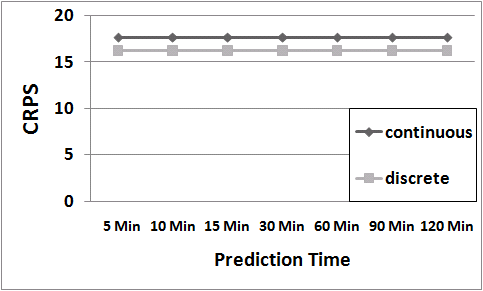
\includegraphics[width = 0.6\columnwidth]{figures/Links_Historic.png}
	}
	\subfigure[Different Start Times]{
		\label{fig:HP2}
		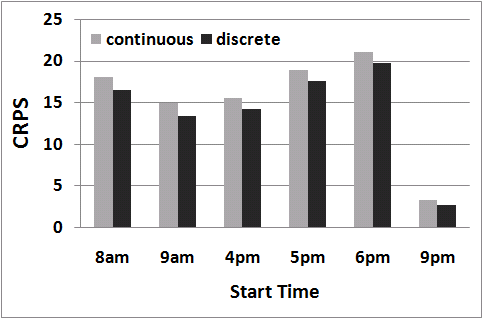
\includegraphics[width = 0.6\columnwidth]{figures/Links_Historic_TOD.png}
	}
	\caption{CRPS Score for HP Approach}\label{fig:HP}
\end{figure}

With the HP approach, we only consider historic data. This means that if we use 8:00am as the \textit{start time}, we consider the travel times at 8:00am across the training days and build the model distribution. Subsequently, we retrieve the actual travel time at 8:00am for each test day and compare it with the model. Since the historic approach is based on historical data only and does not depend on current situation (\textit{query time}), it is consequently independent form the \textit{prediction offset} (\cref{fig:HP1}). \cref{fig:HP2} shows results of the HP approach for different start times in the day with two implications. First, different times of the day are differently hard to predict. In particular the selected standard start times yield much higher CRPS compared to 9:00pm, where there is not too much traffic on the road network and thus not a lot of uncertainty in the prediction.  Second, it shows that the continuous and discrete representation performs rather equivalent. The small difference between the discrete and the continuous case can be explained by the fact that a discrete representation copes better with non-normally distributed link travel times. However, it is important to note that the CRPS of the discrete representation is very sensitive to the discretization interval of the time, i.e., a large discretization interval leads to a larger value of the CRPS and hence not directly comparable to the CRPS of the continuous representation.

Since the results for continuous and discrete link travel times are rather equivalent, for the remainder of the experiments on link travel times we only present results for discrete representation of travel times.

\begin{figure}[h]
    \centering
    \subfigure[Different time horizons]{
        \label{fig:LI1}
        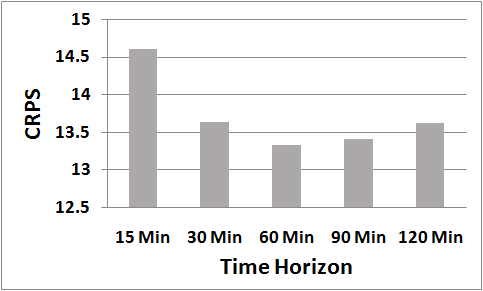
\includegraphics[width = 0.6\columnwidth]{figures/Links_Interpolated_TimeHorizon.png}
    }
    \subfigure[Different values of $\theta$]{
        \label{fig:LI2}
        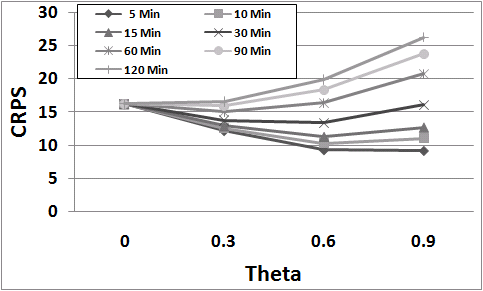
\includegraphics[width = 0.6\columnwidth]{figures/Links_Interpolated_Theta.png}
    }
    \caption{Experiments for the LI approach}\label{fig:LI}
\end{figure}



With regards to the LI approach, we studied the accuracy of the model for
different time horizons $\tau$, ranging from 15 minutes up to 120 minutes. The
results in \cref{fig:LI1} are averaged over all \textit{prediction times} and
clearly show neither of these extremes should be chosen, but rather a good
choice of the time horizon is somewhere in between (i.e., around 60 minutes).
These results are backed up by the experiments shown in \cref{fig:LI2}. In the
LI approach, we eventually use the time horizon to compute $\theta$ as the
weight of the current situation versus historic data. In \cref{fig:LI2} we
directly assign different values to $\theta$. If increasing $\theta$ yields
better results, it means assigning more weight to the current situation is
beneficial and vice versa. \cref{fig:LI2} shows that for prediction times
greater or equal to 60 minutes, increasing $\theta$ results in higher CRPS
scores. Hence we can say, the current situation has no positive influence on the
prediction after 60 minutes, which is the definition of the time horizon
parameter in \cref{subsec:LI}. We use the results in \cref{fig:LI} to conclude
that an optimal time horizon in the Linear Interpolation technique is 60
minutes. Let us note that this is an insightful finding in itself. This result
suggests, that the traffic ``forgets'' its condition an hour ago.

\begin{figure}
	\centering
	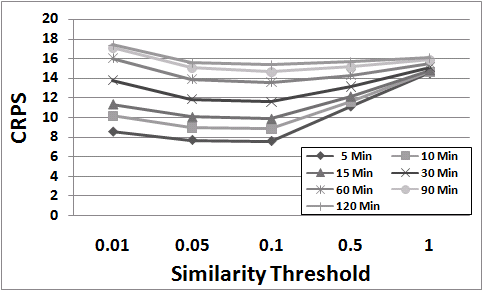
\includegraphics[width = 0.6\columnwidth]{figures/Links_Filtered.png}
	\caption{CRPS Score for SH Approach}\label{fig:SH}
\end{figure}

In the next set of experiments, we evaluate the accuracy of the SH approach. As explained in \cref{subsec:SH}, SH only considers the historical data similar to the current situation. We also defined similarity by the parameter $\lambda$ in \cref{subsec:SH}. We assign different values to $\lambda$ and compare the results.\cref{fig:SH} shows the results. Like LI, SH predicts the near future more accurate than the far future since it is taking the current situation into account. For smaller values of $\lambda$ (e.g., 0.01 \& 0.05) the predictions yield generally higher CRPS. The reason for this behavior is that only very few measurements of the training data meet the similarity
requirement and thus the prediction is based on a possibly non-representative sample. Therefore, as the similarity threshold increases, our model gets more realistic and the results get better. On the other hand, if the similarity
threshold is too loose, data that is not similar to the test day is considered in generating the model, which results in less accurate models.

\begin{figure}[h]
	\centering
	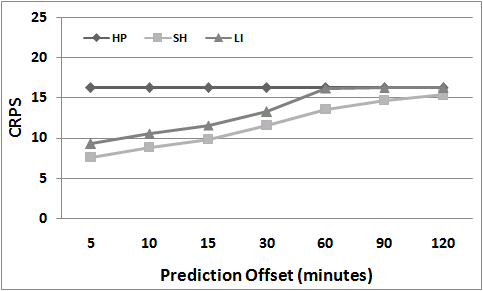
\includegraphics[width = 0.6\columnwidth]{figures/Links_Best.png}
	\caption{CRPS Scores for HP, LI and SH}\label{fig:all_results}
\end{figure}

Finally, we compared the three approaches to each other, using the best setting for the corresponding parameters ($\tau = 60$ minutes and $\lambda = 0.1$). The results are illustrated in \cref{fig:all_results}. Clearly, LI and SH are able to predict the near future more accurately than the farther future, whereas HP is independent from the \textit{prediction offset}. As expected, when $\tau = 60$, for prediction times greater than 60 minutes, LI and HP give the same model. In the following experiments we will use the results of \cref{fig:all_results} to show the important fact that the accuracy of all algorithms proposed to compute a pmf for a route, directly depends on how accurate the probabilistic link travel times are estimated on such route.


\subsection{Route Reliability Computation}
In the following experiments, we apply the techniques for computing
\textit{pltts} to the approaches discussed in \cref{sec:methods}. The first goal
is to evaluate the impact of choosing the right pltt computation technique on
the accuracy of the route pmf. In addition we will assess the effectiveness of
considering the attributes used to classify route computation algorithms in
\cref{sec:methods}.

For these experiments, we use 10 different paths, spanning the road network in
\ref{subsec:Dataset}. The selected paths are 45 miles on average, consisting of
approximately 40 edges. For each path, we use the same standard \textit{start
times} we used for the link travel time predictions. Again, we build a model
with each approach using data from model days and compare the accuracy of the
model with the actual travel time during the test days. Finally, when using the
pltt computation techniques, we only use the optimal parameter discovered in
\cref{subsec:pltt_prediction} for each technique.

\begin{figure}
    \centering
    \subfigure[ConStaInd]{
        \label{fig:ConStaInd}
        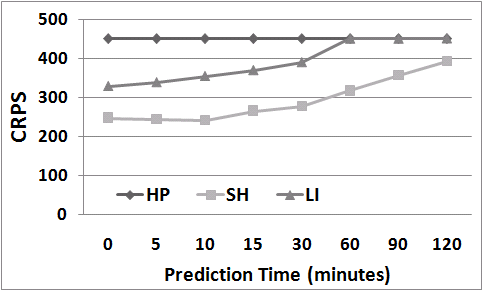
\includegraphics[width = 0.4\columnwidth]{figures/Approaches_ConStaInd.png}
    }
    \subfigure[DisStaInd]{
        \label{fig:DisStaInd}
        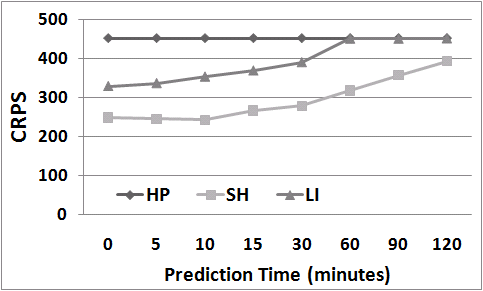
\includegraphics[width = 0.4\columnwidth]{figures/Approaches_DisStaInd.png}
    }
    \subfigure[DisTimInd]{
        \label{fig:DisTimInd}
        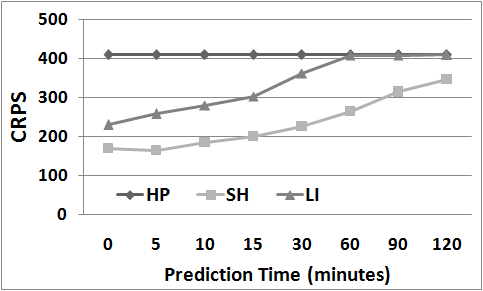
\includegraphics[width = 0.4\columnwidth]{figures/Approaches_DisTimInd.png}
    }
    \subfigure[ConStaCor]{
        \label{fig:ConStaCor}
        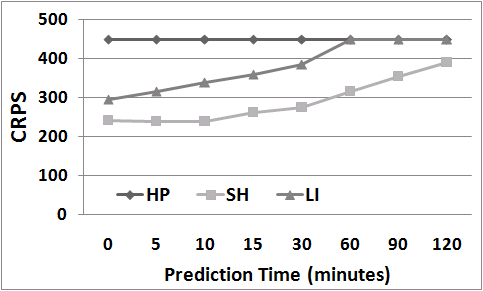
\includegraphics[width = 0.4\columnwidth]{figures/Approaches_ConStaCor.png}
    }
    \caption{Applying pltt computation techniques to route computation algorithms}
    \label{fig:route_pltt}
\end{figure}

As we can see in \cref{fig:route_pltt}, depending on how we model the link travel times, the accuracy of the route pdf (\textbackslash pmf) can vary. Comparing \cref{fig:route_pltt} and \cref{fig:all_results} shows that the accuracy of pltt models \textbf{directly} impact the accuracy of route pmfs. In fact, applying a \textit{good} pltt model to a \textit{bad} route model can yield more accurate models than applying a \textit{bad} pltt model to a \textit{better} route model.

\begin{figure}[h]
	\centering
	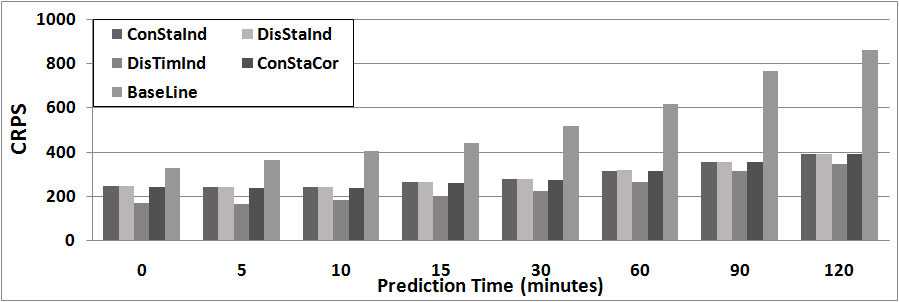
\includegraphics[width = 0.9\columnwidth]{figures/Approaches_All.png}
	\caption{CRPS for probabilistic path computation}\label{fig:path_comp}
\end{figure}

In \cref{fig:path_comp} we put the results of applying the SH approach (\cref{subsec:SH}) to each route computation algorithm side by side. Several observations can be derived from this experiment:

\begin{itemize}
\item Comparing ConStaInd and DisStaInd, we can observe the same characteristics we observed for single links. Representing the link travel times trough a \textit{pmf} or a normal distribution does not drastically change the accuracy of the travel time prediction.
\item  Considering the time-dependency (DisTimInd) however, has a very positive effect on the prediction accuracy, where the results are up to 25\% better compared to the time-independent approaches which have otherwise the same characteristics.
\item The ConStaCor approach is again time-independent and it seems that the consideration of correlation between links does only yield a marginal improvement over the same approach without correlation (ConStaInd). In our experiments, we observe only a 1\%-2\% improvement through the incorporation of correlation in this setting.
\end{itemize}

As an additional comparison partner we included an approach that is used in current route planing systems, named \textit{Baseline}. \textit{Baseline} uses the situation at the \textit{query time} and computes the path travel time without prediction based on the currently available deterministic travel times. The outcome will consequently be a non-probabilistic value as well. The CRPS method allows us to directly compare this approach to the probabilistic counterparts, since it converges to the mean error in the case of certain predictions (i.e., the CRPS can be interpreted as the difference of the prediction and the true value in seconds). The results show that under all settings the probabilistic approaches are superior to the \textit{Baseline} approach which once more justifies the use of probabilistic models in this application.

\begin{figure}
    \centering
    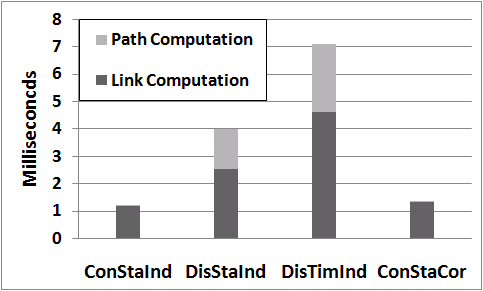
\includegraphics[width = 0.75\columnwidth]{figures/Runtime.png}
    \caption{Runtimes}\label{fig:runtimes}
\end{figure}

Lastly, we evaluated the runtime of all path computation methods discussed in Section \ref{sec:methods}. Runtimes are broken into link travel time prediction and path computation in Figure \ref{fig:runtimes}. Generally, the continuous approaches perform much better due to the analytical nature which yields a much better runtime complexity. As expected, the more complexity we add to the approaches based on a discrete representation, the more costly in terms of computation they become. Link travel time prediction and path computation contribute rather equivalent portions to the runtime in all approaches.
\section{Related Work}
\label{sec:related}
In this section we will review related work on the problem of computing reliability of routes.

\subsection{Deterministic Link Travel Times}
The problem of point-to-point fastest path computation in static road networks
is extensively studied with many precomputation techniques proposed to speed-up
the computation (e.g., \cite{sametcontainer,goldberg05}). These studies
make the simplifying assumption that travel-times of the network edges are single constant deterministic values. As we discussed, in real-world road networks the edge travel-times are time-dependent with a degree of uncertainty, where the arrival-time on an edge determines the
actual travel-time on it. Cooke and Halsey \cite{cooke66tdsp} first studied time-dependent fastest
path probem (TDFP) considering the arrival times to edges. They solved the
problem using Dynamic Programming in discrete time. In \cite{dreyfus69}, Dreyfus
showed that TDFP problem can be solved by a generalization of Dijkstra's method as efficiently as for static fastest path problems.
However, Halpern \cite{halpren77} proved that the generalization of Dijkstra's algorithm is only true for FIFO networks. The FIFO property in road networks ensures that
vehicle-A starting at some node, always arrives at its destination before
vehicle-B, taking the same route at a later time.

In recent years, an increasing number of navigation companies (e.g., Navteq and
Inrix) have started releasing their time-dependent travel-time information for
road networks. With the availability of such datasets, the research community focused on
efficient computation of time-dependent fastest paths and introduced
precomputation techniques (e.g., \cite{Nannicini,timedependentsharc,
timedependentcontraction,DemiryurekSSD11}). The main idea of these
techniques can be grouped in two categories. The first group 
(\cite{Nannicini,DemiryurekSSD11}) proposed  to solve
TDFP with bidirectional A* with different precomputed heuristic functions. On
the other hand, the second group
(\cite{timedependentcontraction,timedependentsharc})  focused on a method that
removes unimportant nodes from the graph without changing the fastest path distances between the remaining (more important) nodes.

% While TDFP approaches yield more accurate paths than that of static algorithms,
% they fall short to capture the inherit uncertainty of the edge travel-times.
% This is because all of the existing time-dependent fastest path algorithms
% model the road network with deterministic time-varying edge
% weights. The travel-times are usually computed by averaging the
% historical travel-times to assign a deterministic cost (i.e., travel-time)
% for each time instance (e.g., for every 15 minutes). There also exists some
% studies that combine the historical and real-time traffic information
% (\cite{PanDS12}) to capture the uncertainty of travel-times and generate
% more up-to-date travel-times. However, the travel-times are still deterministic
% as they are assigned a single value based on the prediction of the short-term
% impact of the real-time traffic.

\subsection{Uncertain Link Travel Times}
\label{subsec:ult}
Uncertainty in databases has attracted a lot of attention from the research
community in the last decade . Many approaches for managing
\cite{AgrBenDasHayetal06,AntJanKocOlt07,JamXuWu08}, querying
\cite{SolIlyCha07,LiSahDes09} and analysing \cite{ChuKaoHun07,ChaCheKaoNr06}
these uncertain datasets have been proposed.
Especially in the field of spatial \cite{CheXiaPra04,DaiYiuMam05} and
spatio-temporal \cite{EmrKriMam12,NieZueEmr13} data, uncertainty was considered
as an important issue due to uncertain sensor measurements or
probabilistic estimations of unknown values. Although these plethora of works
provide many efficient techniques to deal with the uncertainty, only a few works
actually consider how to obtain this uncertainty in a way such that the outcome
of these techniques is meaningful and evaluate the whole end-to-end pipeline of
this process.

Though there exists a large body of work on networks with certain link travel
times, these approaches are not adaptable when the travel times become
uncertain due to sensor failures or predictions of future states of the traffic
network.

The first work \cite{Fra69}  dealing with uncertainty in this context considers
a graph with uncertain edge weights with arbitrary distribution. The particular
interest of this work is to study the characteristics of the probability
distribution describing the length of the shortest path between a source and a
destination.
The author considers the problem from a statistical point of view and no algorithm (besides
a Monte-Carlo driven sampling approach) to compute this distribution is
provided.
The work concludes that (under certain assumptions) the length of the shortest
path is approximately normally distributed. In the end the interesting problem of
comparing two paths is presented. Since a comparison based on the expected
length might not be satisfying the author proposes to compare the paths based on
the probability not to be longer than a parameter $l$. An examplary query
corresponding to this setting would be: \textit{``Which of two possible paths
from my home to work is more likely to let me arrive before 10:00am''}. A
solution is presented under the assumption that the length of a path is normally
distributed.
In contrast to the above work, recent studies have considered more
sophisticated scenarios where the link travel times are not only uncertain but
also time varying and correlated.

\subsubsection{Time-Dependency}
Time dependency of link travel times was recently studied in
large scale traffic networks \cite{DemiryurekSSD11,PanDS12} without uncertainty.
It has been shown that considering the predicted value of a link travel time at the arrival at
that link rather than its value at start of the route vastly improves the accuracy of fastest route
algorithms. One work impressively demonstrating this, is \cite{YuaZhe10} where
the authors utilize historical taxi trajectories in order to learn the
time-dependent travel times of a road network and show the superiority to
routing services like Google or Bing Maps.

Miller-Hooks and Mahmassani first considered stochastic,
time-varying networks where link travel times are independent random variables
with time dependent (discrete) probability distributions \cite{MilEliMah98}.
They address the problem of finding the least possible time path in networks. Specifically, an
algorithm is proposed for determining the least possible travel time from every node to the destination node, its corresponding path and the corresponding probability of
occurrence of that travel time. A sample query would be: \textit{``Regardless
of my starting time, provide me the fastest possible (under best conditions)
route and its corresponding travel time probability from all nodes (intersections) to
work''}. The resulting least possible time path from any starting point may
however have a vanishingly small probability and thus not even be relevant to
the user.

The same authors later addressed the problem of least expected
time (LET) paths under the same settings in \cite{MilMah00}. The problem is to
determine the a priori least expected time paths with the associated expected time from all nodes to
a given destination for each departure time interval
in the period of interest. The sample query would thus slightly differ from the
previous one:\textit{``Provide me the fastest route from all nodes
(intersections) to work under average conditions when starting between 9:00am
and 10:00am''}. In time-invariant stochastic networks this
problem is trivial since it can be reduced to the static case with certain link
travel times by providing each edge with its expected travel time and solving
the shortest path problem using existing methods. In the time variant network
setting however this problem is more complex and two algorithms based on
label-correcting approaches are proposed. The first one provides an exact
solution yielding a worst-case non-polynomial but average polynomial complexity
whereas the second one is more efficient but provides only a lower bound of the
expected travel time and no path information for the LET paths.

In a different study, Nie and Wu \cite{NieWu09} proposed an algorithm for
solving the shortest path problem with on-time arrival reliability (SPOTAR). The SPOTAR problem is to
find the latest possible departure time and the associated route to attain a
given probability of arriving at the destination at a specified arrival time or
earlier. A query example would be: \textit{``What is the latest time I have to
leave home and what path do I have to take to be at work at 10:00am or earlier
with a probability of 90 \%''}. The authors model link travel times by independent
discrete probability distributions and propose an extension to the time-dependent case.
The problem is solved using an exact-label-correcting algorithm whose complexity
is known to be non-deterministic polynomial.

In \cite{CheLamLiSumYan13} the authors assume normally distributed link
travel speeds. They note that some models assume that the travel time depends only
on the arrival time and do not consider the possibility that the travel time might change while the vehicle is on the link. Such models suffer from the drawback that they are not
statistical FIFO consistent. This problem is solved by relaxing this assumption and even allowing
linear correlations between link travel times at consecutive times. In this
case, however, there does not exist a closed form for the exact continuous
distribution of the link travel time, thus a discrete model is proposed. The
ultimate goal is to find the least expected time path (cf \cite{MilMah00})
but between a given source and destination rather than all possible sources. Due
to the problem setting, no probabilistic guarantees (reliability) can be assigned to the resulting path.


\subsubsection{Correlation}
Link travel times in traffic networks are generally dependent on each
other. For example a traffic jam usually extends over several road segments
and a high travel time on one segment usually implies a high travel time on the
next segment. The consideration of correlation between link travel times of
different edges is thus certainly relevant in traffic networks.

In \cite{NieFan06} the authors propose an adaptive path finding strategy for the
stochastic on-time arrival (SOTA). The main idea of SOTA is to provide
the user the route with the highest probability to arrive at the
destination before a given time threshold. A sample query for SOTA is:
\textit{``Which route makes me arrive at work before 10:00am with the highest
probability?''}. They use a discrete model to represent link travel times and consider a simple form of
correlation between adjacent links in which the travel time of an edge is
modeled by two probability mass functions that represent the normal and the
congested state. The states of two adjacent links are then correlated by
conditional probabilities. An algorithm yielding polynomial runtime complexity
is proposed.
Based on the uncertainty model of \cite{NieFan06}, the authors of
\cite{HuaPei10} proposed an approximation algorithm for the probabilistic path
travel time and heuristic approaches to find the best path(s). Though the study
evaluated the approximation error of the inexact approach on a large
real-world dataset they did not evaluate the validity of the exact outcome.

 A similar study \cite{FanKalMoo05} presents an
algorithm based on dynamic programming in order to return the path from a given source to a destination
with the least expected travel time (LET). The link travel times are given by
\textit{pmf}s and correlations are modeled similar to \cite{NieFan06}.

Another work in this direction is \cite{SesSri10}, where the authors consider
the problem of finding the optimal reliability path (ORP), which is equivalent
to the SOTA problem. In their setting the travel time of an edge is normally
distributed and travel times of different edges may correlate without changing
over time. Under these assumptions, subpath optimality (each subpath of the
result path is optimal regarding some criterion) of conventional approaches
does not hold, and hence has to be adapted. Since the proposed algorithm is
also based on a label correcting algorithm, the solution requires the
enumeration of all possible exponential paths in the worst-case. Due to this
characteristic, a fallback solution based on Monte-Carlo sampling is proposed to provide an
approximate solution.

\cite{ZocNieWuMah13} follows the same idea of sampling and provides an
approximate solution using a Monte-Carlo based approach to the SPOTAR (cf
\cite{NieWu09}) problem. Time-dependency is not considered. The main
statement of the simulation based study is that even for the static case, not
considering correlations between edge-weight yields considerably different and unpredictable
results in real-world problems.

\subsubsection{Time-Dependency and Correlation}
Including both, time-dependency and correlation of link travel times for route
optimization problems is generally a very complex undertaking and has only been
considered in very recent studies.

In \cite{DonLiVoVu12}, time-dependent road networks with normally distributed
link travel times and local correlations between them based on two states
(similar to \cite{NieFan06}) are considered. The goal here is to find the path
with the lowest percent variation (PV) between a source and a destination, where
PV is defined by the quotient of the standard deviation and the mean travel time of
the path. The proposed algorithm yields an approximation of the exact result,
but no runtime complexity or runtime experiments are provided.

In \cite{NieWu09a}, the authors extend their previous work \cite{NieWu09} by
introducing limited spatial correlations into the SPOTAR problem - referred to
as reliable apriori shortest path problem (RASP). Specifically, the probability mass function of the traversal time on a link is assumed to be
conditional on the state of that link. The states of a link have a Markovian
property. Namely, the state of present link is dependent on the state of the
link traversed right before arriving at its starting node, and independent of
the links traversed prior to that. The probability distribution of link
traversal times is also allowed to vary over time, which provides a mechanism to
account for the dynamic network behavior such as congestion effects caused by
rush hour traffic. Since the problem is shown to be non-deterministic
polynomial, an approximation algorithm is proposed.

Table \ref{tab:methods} summarizes and categorizes all aforementioned approaches
for handling probabilistic link travel times.

\begin{table}
    \centering
  \begin{tabular}{| l || l | c | c | c | c|}
    \hline
    Ref. & Method & Link model & Time-dep. & Correl. \\
    \hline    \hline
\cite{NieFan06} & SOTA & discrete  & no & yes\\ \hline
\cite{SesSri10} & ORP & normal & no & yes\\ \hline
\cite{NieWu09} & SPOTAR & discrete & yes & no\\ \hline
\cite{NieWu09a} & RASP & discrete & yes & yes\\ \hline
\cite{CheLamLiSumYan13} & LET & normal & no & yes\\ \hline
\cite{ZocNieWuMah13} & SPOTAR & gamma & yes & yes\\ \hline
\cite{DonLiVoVu12} & LET & normal & yes & yes\\ \hline
  \end{tabular}
  \caption{Models considered in this work}
  \label{tab:methods}
  \end{table}


\subsection{Prediction of Link Travel Times}
The prediction of link travel times is an essential part for the
real time computation of the path travel time in a time-dependent
traffic network. Thus, there exist a large body of work that solely
concentrates on techniques solving this problem based on
single link models \cite{PanDS12}, traffic incident models
\cite{PanDemShaGup13}) or Bayesian network models \cite{SunZhaYu06}. Neither
of these approaches does however incorporate the inherent uncertainty of the
predicted values and does not allow for the use of the algorithms discussed in
Section \ref{subsec:ult}. Recently Yang et al.\cite{YanGuoJen13} proposed to
utilize spatio temporal hidden markkov models for this purpose. However the
construction of the model is costly and the prediction
process does not include the current situation in the network which makes the approach hardly
applicable in the real-time setting considered in this work.

\section{Conclusions and Future Work}
\label{sec:conclusion}
In this work we studied the problem of assigning reliability or confidence
values to the estimated travel time of a path in road networks. We showed
that in order to achieve this goal, a whole pipeline of methods has to be
present. We developed three novel methods to obtain probabilistic link
travel times for each link in the network, using historical and
current traffic observations. We presented several methods for summing up
the travel times of each link on a given path under different models. We also
introduced a method for evaluating probabilistic link and path travel time
estimations. This technique made it for the first time possible to compare the
existing approaches and the developed link travel time estimation methods
against each other in terms of accuracy.

The results presented in this paper leave room for improvement and further
investigation. In the current methods, we treated all weekdays as equivalent,
but our observations showed that there is a difference that should be
analyzed and taken into account (e.g. traffic is usually worse on monday
mornings than on other days due to out-of-town commuters). Another important
point for further investigation is the notion of correlation. In following
studies we want to analyse the influence of time-dependent correlations and the
introduction of more possible states of a link. Last, the focus of this work was
mainly on the accuracy comparison of different approaches and thus we assumed
all necessary data to be present in main-memory. However, in a larger setting
this may not be possible and the prediction has to run efficient for the data
to be present in secondary memory database. In this case, we envision
summarization data structures that allow for efficient prediction, based on the
current situation.


\vspace{-0.1in}
\section*{Acknowledgement}
This research has been funded in part by NSF grant IIS-1115153, Caltrans, the USC Integrated Media Systems Center (IMSC), and unrestricted cash gifts from Google, Northrop Grumman, Microsoft, and Oracle. Any opinions, findings, and conclusions or recommendations expressed in this material are those of the author(s) and do not necessarily reflect the views of any of the sponsors such as the National Science Foundation.

\begin{scriptsize}
%\begin{footnotesize}
\bibliographystyle{IEEEtran}
\bibliography{roadnetworks}
%\end{footnotesize}
\end{scriptsize}

\end{document}
